%\section{Introducci�n}
%\subsection{Motivaci�n}
El etiquetado o anotado gramatical, tambi�n conocido como Part-of-speech tagging, POS tagging o simplemente POST, es el proceso de asignar una etiqueta gramatical a cada una de las palabras de un texto seg�n su categor�a l�xica. Como se menciona m�s adelante, el etiquetado gramatical juega un papel importante en  �reas de la linguistica computacional como por ejemplo s�ntesis del habla, reconocimiento del habla y recuperaci�n de la informaci�n.

Este proceso es realizado manualmente por linguistas o autom�ticamente mediante programas conocidos como etiquetadores gramaticales. Estos programas son entrenados con el objetivo de que aprendan a etiquetar. Este entrenamiento se realiza utilizando un corpus anotado previamente denominado corpus de entrenamiento. De esta manera el etiquetador obtiene, procesa y retiene informaci�n sobre como est� anotado el corpus de entrenamiento que utiliza posteriormente durante el proceso de etiquetaci�n gramatical. 

Una vez finalizado el entrenamiento, se procede a etiquetar el texto requerido utilizando la informacion adquirida.

Basicamente un corpus etiquetado o anotado es una lista de palabras con su correspondiente etiqueta gramatical. Por ejemplo:
\\ \\
A			DT\\
form			NN\\
of			IN\\
asbestos		NN\\
once			RB\\
used			VBN\\
to			TO\\
make			VB\\
Kent			NNP\\
cigarette		NN\\
filters			NNS\\
has			VBZ\\
caused			VBN\\
a			DT\\
high			JJ\\
percentage		NN\\
of			IN\\
cancer			NN\\
deaths			NNS\\
among			IN\\
a			DT\\
group			NN\\
of			IN\\
workers			NNS\\
exposed			VBN\\
to			TO\\
it			PRP\\
more			RBR\\
than			IN\\
30			CD\\
years			NNS\\
ago			RB\\
,			,\\
researchers		NNS\\
reported		VBD\\
.			.\\ \\

La complejidad del etiquetado gramatical reside en que la etiqueta no depende solo de la palabra o tipo de palabra que se est� etiquetando, por el contrario, la ubicaci�n y el contexto de la palabra en donde �sta aparece es un factor determinante al asignar la etiqueta correspondiente.

Como fu� mencionado anteriormente, la etapa de entrenamiento de un etiquetador gramatical obtiene, procesa y retiene informaci�n sobre el contexto y la ubicaci�n de una palabra y la etiqueta asignada. Luego se utiliza esta informaci�n en el proceso de etiquetacion, donde el etiquetador analiza para cada palabra su ubicaci�n y contexto, y en base a ello y al conocimiento adquirido previamente con el corpus de entrenamiento determina una etiqueta gramatical.

Uno de los grandes problemas del etiquetado gramatical reside en la falta de corpus anotados para utilizar durante el entrenamiento.

Los corpus etiquetados (tambi�n llamados corpus de entrenamiento) son etiquetados manualmente por linguistas especializados. Es un trabajo profundamente meticuloso y tedioso ya que el linguista debe dar una etiqueta gramatical palabra por palabra, en corpus del orden del MILLON de palabras. Ademas de lo tedioso y complejo del trabajo, el tiempo empleado para etiquetar un corpus es sumamente extenso y como consecuencia el valor economico es realmente alto, ya que intervienen grupos de trabajo altamente capacitados durante un tiempo prolongado.

El resultado de este complejo proceso artesanal es una tabla de palabras con su correspondiente etiqueta gramatical como se mostr� anteriormente. Ante la importancia que adquieren los corpus etiquetados es inevitable pensar en alg�n otro tipo de texto que posea informaci�n de etiquetas. 

Por ejemplo un diccionario contiene una palabra, su definici�n y algunos ejemplos en donde �sta aparece con cada uno de sus sentidos. Es decir que de alguna manera un diccionario contiene por cada palabra uno o m�s contextos en donde �sta aparece etiquetada. Entonces si tomamos todos los ejemplos de cada palabra de un diccionario y su etiqueta podemos construir un corpus parcialmente anotado. 

\subsection{Trabajo realizado}
La idea de este trabajo es suplir la falta de corpus de enternamiento utilizando la informaci�n de etiquetado que posee un diccionario como una nueva fuente de informaci�n para entrenar etiquetadores autom�ticos. Utillizar esta informaci�n existente para etiquetar, medir y comparar resultados en el rendimiento conseguido. Combinar e integrar esta informaci�n obtenida con corpus de entrenamiento cl�sicos e inspeccionar resultados en el etiquetado.
Este trabajo menciona detalladamente la forma de extraer la informaci�n relevante de etiquetas gramaticales a partir de un diccionario y las decisiones que fueron aplicadas.
Por �ltimo se realizan mediciones entre esta nueva fuente de informaci�n y los corpus cl�sicos de entrenamiento y se presentan las conclusiones.



%
Como se mencion� anteriormente, el etiquetado gramatical es el proceso de asignar una etiqueta a cada una de las palabras de un texto seg�n su categor�a l�xica. O expresado de otra manera: dada una secuencia de palabras como entrada, obtener como salida una secuencia de etiquetas para las mismas. Este proceso se realiza en base a la definici�n de la palabra y al contexto en que �sta aparece. \\

\noindent Por ejemplo en:\\

\emph{Does that flight serve dinner} \\

\noindent \emph{dinner} es un sustantivo y por lo tanto recibe la etiqueta para sustantivos NN.\\

El etiquetado gramatical brinda una gran cantidad de informaci�n sobre una palabra y sus vecinas. Por ejemplo, las etiquetas distinguen entre pronombres posesivos (mi, tu, su, �tc.) y pronombres personales (Yo, T�, �l, �tc.). Saber si una palabra es un pronombre posesivo o personal nos brinda informaci�n sobre las palabras que pueden ocurrir a continuaci�n: los pronombres posesivos generalmente son sucedidos por un sustantivo (como en \emph{Mi comida}) mientras que los personales son sucedios por un verbo (como en \emph{Yo duermo}). 

Utilizando esta deducci�n podemos aseverar que si una palabra fu� etiquetada como pronombre personal, es muy probable que la pr�xima palabra sea un verbo. 
Una etiqueta gramatical tambi�n puede ofrecer informaci�n relacionada con la pronunciaci�n de la palabra. En ingl�s la palabra \emph{content} puede ser un sustantivo o un adjetivo y su pronunciaci�n var�a dependiendo de este hecho. Utilizando estas ideas se pueden producir pronunciaciones m�s naturales en un sistema de s�ntesis del habla (texto a voz) o tambi�n se puede obtener m�s exactitud en un sistema de reconocimiento del habla (voz a texto).

Otra aplicaci�n importante del etiquetado gramatical en sistemas de recuperaci�n de la informaci�n es el reconocimiento de sustantivos u otro tipo de palabras importantes dentro de un documento, para guardar y utilizar esta informaci�n en b�squedas posteriores. 

Por �ltimo, la asignaci�n autom�tica de etiquetas gramaticales juega un papel importante en algoritmos de desambig�aci�n del sentido de la palabra y en modelos ling��sticos basados en n-gramas utilizados en sistemas de reconocimiento del habla.

%\section{Definiciones y marco te�rico}	
A continuaci�n se presentan definiciones y teor�as sobre las que se basa el trabajo realizado. Se presenta el concepto de etiqueta gramatical, es decir, un c�digo que identifica el rol que cumple una palabra dentro de cierto contexto. Se muestran los conjuntos de etiquetas que han sido utilizados intentando abarcar los distintos significados que pueden tener las palabras. Se explica el concepto de etiquetado gramatical, es decir, la tarea de asignar a cada palabra una etiqueta gramatical adecuada seg�n el contexto en donde �sta aparece. Se muestran ejemplos de que esta tarea est� muy lejos de ser trivial, introduciendo el concepto de ambig�edad gramatical. 

Se exhibe la importancia del etiquetado gramatical dentro de distintas �reas como la computaci�n ling�istica, reconocimiento y s�ntesis del habla. Se muestra como se maneja este proceso utilizando programas que lo realizan autom�ticamente; los etiquetadores gramaticales autom�ticos. Se decriben implementaciones actuales que utilizan informaci�n estad�stica que el etiquetador utiliza para reproducir el etiquetado.
 
Se presenta el concepto de corpus y corpus anotado gramaticalmente como conjuntos de informaci�n extremadamente valiosos para todas estas tareas.
Se muestra la forma de medir, evaluar y comparar el rendimiento de los etiquetadores gramaticales, introduciendo los conceptos de corpus de entrenamiento y corpus de verificaci�n. Se muestran t�cnicas de an�lisis de error para la etiquetaci�n autom�tica. Se exhibe tambi�n el manejo de ciertos casos especiales dentro del proceso de etiquetaci�n autom�tico; las palabras desconocidas. Y por �ltimo se explican en detalle los etiquetadores autom�ticos utilizados en el presente trabajo.
%\subsection{Etiquetas} 
Tradicionalmente la deficinici�n de POS o etiqueta gramatical se ha basadado en funciones sint�cticas y morfol�gicas, es decir que se agrupan en clases las palabras que funcionan similarmente con respecto a lo que puede ocurrir a su alrededor (sus propiedades de distribuci�n sint�ctica) o con respecto a los afijos que poseen (sus propiedades morfol�gicas). Mientras que las clases de palabras tienen tendencia hacia la coherencia sem�ntica (por ejemplo los sustantivos generalmente describen gente, lugares o cosas y los adjetivos generalmente describen propiedades), este no es necesariamente el caso y en general no se utiliza coherencia sem�ntica como criterio para la definici�n de POS o etiqueta gramatical.

Las etiquetas gramaticales pueden ser divididas en dos grandes categor�as: clases cerradas y clases abiertas. Las clases cerradas son aquellas que tienen miembros relativamente fijos. Por ejemplo, las preposiciones son una clase cerrada en porque hay un conjunto cerrado de ellas, es decir que son un grupo de palabras que raramente var�a ya que raramente se agregan nuevas preposiciones. En contraste, los sustantivos y los verbos son clases abiertas ya que continuamente se introducen y eliminan nuevos verbos y sustantivos al lenguaje. Es probable que cualquier hablante o corpus tenga una clase abierta de palabras diferente, pero todos los hablantes de un lenguaje y corpora suficientemente grandes, seguramente van a compartir el conjunto de clases de palabras cerradas. Las clases de palabras cerradas tambi�n son generalmente palabras funcionales como \textsl{de}, \textsl{y} o \textsl{tu}, que tienden a ser muy cortas, ocurrir frecuentemente y generalmente tienen usos estructurales en gram�tica.

Hay cuatro clases abiertas principales: 
\begin{itemize}
	\item \textbf{Sustantivos }
	Es el nombre dado a la clase sint�ctica que denota personas, lugares o cosas. Pero desde que las clases sint�cticas como sustantivos son definidas sint�ctica y morfol�gicamente en vez que sem�nticamente, algunas palabras para personas, lugares y cosas pueden no ser sustantivos y a la inversa, algunos sustantivos pueden no ser palabras para personas, lugares o cosas. Por lo tanto los sustantivos incluyen t�rminos concretos como \textsl{barco} y \textsl{silla}, abstracciones como \textsl{banda ancha} y \textsl{relaci�n}. Se puede definir a una palabra como  sustantivo bas�ndose en caracter�sticas como la capacidad de ocurrir con determinantes (una \textsl{cabra}, su \textsl{banda ancha}), tomar posesivos (los ingresos anuales de \textsl{IBM}) y para la mayor�a pero no todos los sustantivos, ocurrir en la forma plural (\textsl{cabras}, \textsl{tel�fonos}).
Los sustantivos tradicionalmente son agrupados en sustantivos propios y sustantivos comunes. 
\begin{itemize}
	\item \textbf{Sustantivos propios:} Son nombres de personas espec�ficas o entidades y usualmente son escritos en may�scula.
	\item \textbf{Sustantivos comunes:} En algunos lenguajes se dividen en sustantivos contables e incontables.
		\begin{itemize}
			\item \textbf{Sustantivos contables:} Son aquellos que permiten establecer su n�mero en unidades. En general esta clase posee forma singular y plural (silla/s, dedo/s). 
			\item \textbf{Sustantivos incontables:} Se refieren a sustantivos que no se puede determinar su n�mero en unidades (harina, nieve, az�car).
		\end{itemize}
\end{itemize}

\item \textbf{Verbos:} Los verbos son una clase de palabras que incluye a la mayor�a de las palabras referidas a acciones y procesos. Tienen ciertas formas morfol�gicas  como tiempo, modo, persona, regularidad, �tc. Adem�s, el verbo puede concordar en g�nero, persona y n�mero con algunos de sus argumentos o complementos (a los que normalmente se conoce como sujeto, objeto, �tc.). En espa�ol concuerda con el sujeto siempre en n�mero y casi siempre en persona (la excepci�n es el caso del llamado sujeto inclusivo: \textsl{Los espa�oles somos as�}).

Algunos ejemplos: \\ \\
Marisol \textsl{canta} una �pera.\\
La comida \textsl{est�} caliente.\\

\item \textbf{Adjetivos:} Las palabras pertenecientes a esta clase expresan propiedades o cualidades. Por ejemplo
\textsl{Ese hombre es \textbf{alto}}. Los adjetivos tienen g�nero y n�mero al igual que los sustantivos. El g�nero y el n�mero de los adjetivos depende del sustantivo al que acompa�an. Hay adjetivos que presentan una sola forma para el masculino y para el femenino. Son adjetivos de una sola terminaci�n (verde, especial, amable, grande, �tc.). Por el otro lado, los adjetivos de dos terminaciones presentan distintas formas para el masculino y el femenino (feo-fea, peque�o-peque�a, blanco-blanca, �tc.)
Se clasifican en: 
\begin{itemize}
	\item \textbf{Determinativos:} Preceden al sustantivo, lo concretan y lo presentan
		\begin{itemize}
			\item \textbf{Demostrativos:} \textsl{Esta} ni�a
			\item \textbf{Posesivos:} \textsl{Mi} ni�a
			\item \textbf{Numerales:} \textsl{Tres} ni�as
			\item \textbf{Indefinidos:} \textsl{Algunas} ni�as
			\item \textbf{Exclamativos:} �\textsl{Qu�} ni�a!
			\item \textbf{Interrogativos:} �\textsl{Qu�} ni�a?
		\end{itemize}
	\item \textbf{Calificativos:} Califican al sustantivo, es decir, a�aden cualidades al sustantivo. Los adejtivos calificativos se dividen en especificativos y explicativos o ep�tetos.
		\begin{itemize}
			\item \textbf{Adejtivos calificativos especificativos:} Son aquellos que concretan el significado del sustantivo. Suelen aparecer detr�s del sustantivo.\\
Ej: Quiero una corbata \textsl{azul}.

			\item \textbf{Adejtivos calificativos explicativos o ep�tetos:} indican cualidades que ya de por s� lleva el sustantivo. Suelen ir delante del sustantivo.\\
Ej: \textsl{Blanca} nieve, \textsl{Verde} hierba.\\
		\end{itemize}
\end{itemize}
\item \textbf{Adverbios:} Los adverbios son otro ejemplo de clase abierta de palabras: se definen como modificadores del verbo, adjetivo o de otro adverbio. Tradicionalmente se dividen en:
\begin{itemize}
	\item \textbf{Adverbios de lugar}: aqu�, all�, ah�, all�, ac�, arriba, abajo, cerca, lejos, delante, detr�s, encima, debajo, enfrente, atr�s, alrededor, etc.
\item \textbf{Adverbios de tiempo absoluto}: pronto, tarde, temprano, todav�a, a�n, ya, ayer, hoy, ma�ana, siempre, nunca, jam�s, pr�ximamente, prontamente, anoche, enseguida, ahora, mientras.
\item \textbf{Adverbios de modo}: bien, mal, regular, despacio, deprisa, as�, tal, como, aprisa, adrede, peor, mejor, fielmente, estupendamente, f�cilmente - todas las que se formen con las terminaciones "mente".
\item \textbf{Adverbios de cantidad o grado}: muy, poco, muy poco, mucho, bastante, m�s, menos, algo, demasiado, casi, s�lo, solamente, tan, tanto, todo, nada, aproximadamente.
\end{itemize}
\end{itemize}

Por otro lado tenemos las clases cerradas de palabras. Primero hacemos una vista r�pida para luego definirlas con m�s detalle:
\begin{itemize}
	\item \textbf{Preposiciones:} Las preposiciones son enlaces que relacionan los componentes de una oraci�n para brindarles sentido. La uni�n se lleva a  cabo con una o varias palabras. La significaci�n que dan las preposiciones responde a circunstancias de movimiento, lugar, tiempo, modo, causa, posesi�n, pertenencia, materia y procedencia.\\
Algunos ejemplos:\\ \\
Me levant� de la cama \textbf{a} las ocho de la ma�ana.\\
Dej� mis cuadernos \textbf{sobre} el sill�n.\\
Corr� apresurado \textbf{hacia} la calle pero no logr� divisarte. \\
Luc�a se divierte \textbf{con} sus mu�ecas.\\
	\item \textbf{Determinantes:} Los determinantes son clases cerradas de palabras que ocurren con sustantivos, generalmente marcando el principio de una frase sustantiva. Un peque�o subtipo de determinantes es el art�culo: \textsl{a}, \textsl{el}. Otros determinantes incluyen \textsl{ese} (como en \textsl{el libro ese}).
	\item \textbf{Pronombres:} Los pronombres son formas que generalmente act�an como una clase de atajo para referirse a alguna frase sustantiva, entidad o evento. Los \textbf{pronombres personales} hacen referencia a personas o entidades (Yo, t�, �l, ella, nosotros, ellos, �tc.), Los \textbf{pronombres posesivos} son formas de pronombres personales que indican una posesi�n actual o mas generalmente solo una relacion abstracta entre la persona y algun objeto (m�o, tuyo, suyo, mi, nuestro, �tc.)
	\item \textbf{Conjunciones:} Las conjunciones son utilizadas para unir dos frases, cl�usulas o sentencias. Las conjunciones coordinantes como \textsl{y}, \textsl{o} unen dos elementos de igual estado. Las conjunciones subordinativas son utilizadas cuando uno de los elementos es de alg�n tipo de estado integrado. Por ejemplo \textsl{Me molest� \textbf{que} no me lo dijeras}.
	\item \textbf{Verbos auxiliares:} Los verbos auxiliares son verbos que proporcionan informaci�n gramatical y sem�ntica adicional a un verbo de significado completo. Dichos verbos auxiliares brindan la informaci�n gramatical de modo, tiempo, persona y n�mero y las formas no personales. Por ejemplo \textsl{�por qu� no \textbf{has} llegado a la hora prevista? } o tambi�n \textsl{La avenida principal de la ciudad \textbf{fue} clausurada por obras de refacci�n}.
	\item \textbf{Numerales:} Los determinantes numerales simplemente numerales son los que expresan de modo preciso y exacto la cantidad de objetos designados por el sustantivo al que acompa�an, delimitan o designan. Limitan el significado general del sustantivo, precisando con exactitud la cantidad de objetos que aquel designa o el lugar de orden que ocupan. Los numerales pueden ser de varias clases. Los m�s importantes son:\\ \\
	\begin{itemize}
\item \textbf{Cardinales}: informan una cantidad exacta:\\
Quiero \textsl{cuatro} libros.
\item \textbf{Ordinales}: informan del orden de colocaci�n:\\
Quiero el \textsl{cuarto} libro.
\item \textbf{Fraccionarios}: informan de particiones de la unidad:\\
Quiero la \textsl{cuarta} parte.
\item \textbf{Multiplicativos}: informan de m�ltiplos:\\
Quiero \textsl{doble} raci�n.
\end{itemize}
\end{itemize}





 
\subsection{Conjuntos de etiquetas} 
La secci�n anterior di� una descripci�n general de los tipos de clases sint�cticas a las que pertenecen las palabras. Esta secci�n presenta los conjuntos de c�digos que se corresponden con cada una de estas clases sint�cticas, tambi�n llamados \textsl{tagsets} o conjuntos de etiquetas. 

Todav�a no existe un consenso sobre el conjunto de etiquetas o \textsl{tagset} m�s adecuado. Generalmente los conjuntos de etiquetas grandes ofrecen una decripci�n sint�ctica m�s espec�fica mientras que los conjuntos de etiquetas m�s peque�os usualmente brindan una informaci�n ling��stica m�s acotada. Una de las caracter�sticas clave para decidir que conjunto de etiquetas es el m�s adecuado justamente depende del nivel de detalle ling��stico que se est� buscando. 

Tambi�n cabe destacar que los conjuntos de etiquetas m�s peque�os generalmente est�n contenidos en los conjuntos mayores. Debido a que las etiquetas m�s espec�ficas que se encuentran en los conjuntos mayores pueden ser convertidas en etiquetas de menor especificidad con la consecuente p�rdida de detalle ling��stico. 

Por el otro lado, tambi�n se pueden convertir las etiquetas pertenecientes a un conjuntos peque�os en etiquetas de mayor especificidad que pertenecen a conjuntos m�s grandes, ya que generalmente existen etiquetas equivalentes en estos �ltimos.

A continuaci�n se muestra como ejemplo el conjunto de etiquetas \textsl{Penn Tree Bank}:

\begin{center}
\begin{longtable}{| l | l | l |}
\caption{Conjunto de Etiquetas Penn Tree Bank}
	\hline
\textbf{Etiqueta}	&	\textbf{Descripci�n}	&	\textbf{Ejemplo}\\
\hline
\endhead
\hline
\endfoot
\endlastfoot
	\hline
CC & Coordinating conjunction &\textsl{and}\\
CD & Cardinal number &\textsl{1, third}\\
DT & Determiner &\textsl{the}\\
EX & Existential &\textsl{there there is}\\
FW & Foreign word &\textsl{d'hoevre}\\
IN & Preposition/subordinating conjunction &\textsl{in, of, like}\\
JJ & Adjective  &\textsl{green}\\
JJR & Adjective, comparative &\textsl{greener}\\
JJS & Adjective, superlative &\textsl{greenest}\\
LS & List marker  &\textsl{1)}\\
MD & Modal  &\textsl{could, will}\\
NN & Noun, singular or mass &\textsl{table}\\
NNS & Noun plural  &\textsl{tables}\\
NNP & Proper noun, singular &\textsl{John}\\
NNPS & Proper noun, plural &\textsl{Vikings}\\
PDT & Predeterminer both &\textsl{the boys}\\
POS & Possessive ending &\textsl{friend's}\\
PRP & Personal pronoun &\textsl{I, he, it}\\
PRP\$ & Possessive pronoun &\textsl{my, his}\\
RB & Adverb &\textsl{however, usually, naturally, here, good}\\
RBR & Adverb, comparative &\textsl{better}\\
RBS & Adverb, superlative &\textsl{best}\\
RP & Particle &\textsl{give up}\\
SYM & Symbol &\textsl{+,\%,\&}\\
TO & To &\textsl{to go, to him}\\
UH & Interjection &\textsl{uhhuhhuhh}\\
VB & Verb, base form &\textsl{take}\\
VBD & Verb, past tense &\textsl{took}\\
VBG & Verb, gerund/present participle &\textsl{taking}\\
VBN & Verb, past participle &\textsl{taken}\\
VBP & Verb, sing. present, non-3d &\textsl{take}\\
VBZ & Verb, 3rd person sing. present &\textsl{takes}\\
WDT & Wh-determiner &\textsl{which}\\
WP & Wh-pronoun &\textsl{who, what}\\
WP\$ & Possessive wh-pronoun &\textsl{whose}\\
WRB & Wh-abverb  &\textsl{where, when}\\
\$ & Dollar sign &\textsl{\$}\\
\# & Pound sign &\textsl{\#}\\
" & Left quote &(' or ")\\
" & Right quote &(' or ")\\
( & Left parenthesis &( [, (, \{, <)\\
) & Right parenthesis &( ], ), \}, >)\\
, & Comma &,\\
. & Sentence-final punc &( . ! ?)\\
: & Mid-sentence punc &( : ; ... -)\\
\hline
\end{longtable}
\end{center}
Aunque no exista un consenso sobre que conjunto de etiquetas utilizar, hay un peque�o n�mero de conjuntos de etiquetas o \textsl{tagsets} populares para el idioma ingl�s, muchos de los cuales evolucionaron a partir del conjunto de etiquetas utilizado para etiquetar el corpus \textsl{Brown}. Este conjunto de etiquetas se conoci� como el \textsl{Brown Corpus Tag-set}, un conjunto de 87 etiquetas que se utiliz� para etiquetar el corpus \textsl{Brown}.

Junto al \textsl{Brown Corpus Tag-set} se encuentran dos de los conjuntos de etiquetas m�s utilizados: el conjunto de etiquetas reducido \textsl{Pen Treebank} de 45 etiquetas y el conjunto de etiquetas \textsl{CLAWS C5} de tama�o medio (62 etiquetas) que fu� utilizado para etiquetar el \textsl{British National Corpus} (BNC).

El conjunto de etiquetas \textsl{Penn Treebank} mostrado en la tabla anterior fu� utilizado para etiquetar el corpus \textsl{Brown}, el corpus \textsl{Wall Street Journal} y el corpus \textsl{Switchboard} entre otros. En realidad, quiz�s en parte por su peque�o tama�o es uno de los conjuntos de etiquetas m�s utilizado. 

A continuaci�n se exhiben algunos ejemplos de oraciones del corpus \textsl{Brown} etiquetadas con el conjunto de etiquetas \textsl{Penn Treebank}. Se representar� una palabra etiquetada mediante la colocaci�n de una barra oblicua seguida de su etiqueta:
{\small \begin{enumerate}
	\item The/DT grand/JJ jury/NN commented/VBD on/IN a/DT number/NN of/IN other/JJ topics/NNS ./.
	\item \textbf{There/EX} are/VBP 70/CD children/NNS \textbf{there/RB}
	\item Although/IN preliminary/JJ findings/NNS were/VBD \textbf{reported/VBN} more/RBR than/IN a/DT year/NN aho/IN ,/, the/DT latest/JJS results/NNS appear/VBP in/IN today/NN \textbf{'s/POS} New/NNP England/NNP Journal/NNP of/IN Medicine/NNP ./.
\end{enumerate}
}
El primer ejemplo exhibe los determinantes \textsl{the} y \textsl{a}, los adjetivos \textsl{grand} y \textsl{other}, los sustantivos comunes \textsl{jury}, \textsl{number} y \textsl{topics} y el verbo en tiempo pasado \textsl{commented}. 

El segundo ejemplo muestra el uso de la etiqueta ET para marcar la construcci�n existencial \textsl{there} y otro uso de \textsl{there} que es etiquetado como un adverbio (RB). 

El tercer ejemplo muestra la segmentaci�n del morfema posesivo \textsl{'s} y un ejemplo de la construcci�n pasiva 'were reported', en la cual el verbo \textsl{reported} est� marcado como un pasado participio (VBN) en vez de como un pasado simple (VBD). Tambi�n es interesante notar que el sustantivo propio \textsl{New England} est� etiquetado como NNP. Finalmente, se puede observar que como \textsl{New England Journal of Medicine} es un sustantivo propio, el etiquetado de \textsl{Treebank} elige marcar cada sustantivo separado como NNP, incluyendo \textsl{journal} y \textsl{medicine}, que en otro caso hubieran sido etiquetados como sustantivos comunes (NN).

\subsubsection{Especificidad de etiquetas: Treebank vs C5 y Brown} 
El conjunto de etiquetas \textsl{Penn Treebank} es una selecci�n de 45 etiquetas del conjunto de etiquetas \textsl{Brown} (de 87 etiquetas). Este conjunto reducido excluye cierta informaci�n ling��stica. Por ejemplo los conjuntos de etiquetas \textsl{Brown} y \textsl{C5} incluyen una etiqueta para cada una de las diferentes formas de los verbos \textsl{do}, \textsl{be} y \textsl{have}(C5 propone la etiqueta VDD para \textsl{did} y VDG para \textsl{doing}). Estas etiquetas fueron omitidas en el conjunto \textsl{Penn Treebank}.

Ciertas distinciones sint�cticas no fueron marcadas en el conjunto de etiquetas \textsl{Penn Treebank}. Por ejempo, la etiqueta IN es utilizada para preposiciones para conjunciones subordinadas. El conjunto del \textsl{Penn Treebank} no es suficientemente espec�fico en ciertos casos. Los conjuntos de etiquetas de \textsl{Brown} y \textsl{C5}, por ejemplo, distinguen preposiciones (IN) de conjunciones subordinadas (CS), como en los siguiente ejemplos:
{\small \begin{enumerate}
	\item \textbf{after/CS} spending/VBG a/AT few/AP days/NNS at/IN the/AT Brown/NP Palace/NN Hotel/NN
	\item \textbf{after/IN} a/AT wedding/NN trip/NN to/IN Corpus/NP Christi/NP ./.
\end{enumerate} }
Tambi�n tienen dos etiquetas para la palabra \textsl{to}; en \textsl{Brown} el uso del infinitivo es etiquetado como TO, mientras que las preposiciones son etiquetadas como IN:
{\small \begin{enumerate}
	\item \textbf{to/TO} give/VB priority/NN \textbf{to/IN} teacher/NN pay/NN raises/NNS
\end{enumerate} }
El conjunto de etiquetas \textsl{Brown} tambi�n posee la etiqueta NR para sustantivos adverbiales como \textsl{home}, \textsl{west}, \textsl{Monday} y \textsl{tomorrow}. Como \textsl{Penn Treebank} carece de esta etiqueta; \textsl{Monday}, \textsl{Tuesday} y otros d�as de la semana son marcados como NNP, \textsl{tomorrow}, \textsl{west} y \textsl{home} son marcados algunas veces como NN y algunas veces como RB. Esto hace al conjunto de etiquetas \textsl{Penn Treebank} menos �til para tareas de alto nivel ling��stico como la detecci�n del tiempo de frases.

Sin embargo, el conjunto de etiquetas \textsl{Penn Treebank} ha sido el m�s utilizado para la evaluaci�n de algoritmos de etiquetado autom�tico. Esta es la raz�n por la cual elegimos este conjunto de etiquetas para utilizar en el desarrollo del presente trabajo. 
%\subsection{Corpus}
%Un corpus es una colecci�n o cuerpo de textos en formato electr�nico. El plural es corpora. 
%\subsection{Etiquetadores gramaticales autom�ticos} 
Como se mencion� anteriormente, el etiquetado gramatical es el proceso de asignar una etiqueta gramatical a cada palabra dentro de un texto. Generalmente las etiquetas gramaticales tambi�n son aplicadas a los signos de puntuaci�n, por lo tanto el etiquetado requiere que los signos de puntuaci�n sean separados de las palabras. Este proceso se realiza previamente o como parte del etiquetado y es conocido como \textsl{tokenizaci�n}; es el proceso encargado de separar puntos, comas, par�ntesis y otros caracteres de las palabras as� como tambi�n desambiguar el fin de oraci�n (por ejemplo un punto o signo de pregunta) de un signo de puntuaci�n (como en una abreviaci�n por ejemplo \textsl{�tc.})

La entrada para un algoritmo de etiquetaci�n autom�tica es una cadena de palabras y un conjunto de etiquetas. La salida es la mejor etiqueta encontrada para cada palabra.
Consideremos  las siguientes oraciones etiquetadas gramaticalmente:
\\
\\
\textsl{Book/VB that/DT flight/NN ./.\\
Does/VBZ that/DT flight/NN serve/VB dinner/NN ?/.}
\\
\\
Asginar una etiqueta gramatical a una palabra no es una tarea trivial incluso en estos sencillos ejemplos. Por ejemplo, la palabra \textsl{book} es ambigua. Es decir que tiene m�s de un uso posible y por lo tanto m�s de una etiqueta gramatical posible. Puede ser un verbo (como en \textsl{\textbf{book} that flight} o \textsl{to \textbf{book} the suspect}) o un sustantivo (como en \textsl{hand me that \textbf{book}} o \textsl{a \textbf{book} of matches}). An�logamante \textsl{that} puede ser un determinante (como en \textsl{Does \textbf{that} flight serve dinner}) o un complementador (como en \textsl{I thought \textbf{that} your flight was earlier}). 

El problema del etiquetado gramatical reside en resolver estas ambiguedades, eligiendo la etiqueta adecuada seg�n el contexto. 
�Pero qu� magnitud tiene el problema de la ambiguedad de las palabras? Podemos apreciar que la mayor�a de las palabras en ingl�s no son ambiguas, o l o que es lo mismo, tienen una �nica etiqueta posible. Pero sin embargo muchas de las palabras m�s comunes del ingl�s son ambiguas, es decir que las palabras m�s utilizadas, las que se emplean con mayor frecuencia, pueden tener m�s de una etiqueta. Por ejemplo \textsl{can} puede ser un auxiliar (puede), un sustantivo (lata o contenedor de metal) o un verbo (poner algo en la lata).

Afortunadamente muchas de las palabras ambiguas son f�cilmente desambiguables. Esto sucede porque las etiquetas asociados a una palabra no suelen ocurrir con la misma frecuencia. Por ejemplo \textsl{a} puede ser un determinante o la letra \textsl{a} (quiz�s como parte de un acr�nimo o una inicial), pero es preciso notar que el sentido de \textsl{a} es mucho m�s frecuente como determinante que como letra. Es decir que es mucho m�s frecuente encontrar \textsl{a} en oraciones como \textsl{My father bought \textbf{a} new car} o \textsl{There is \textbf{a} hair in my soup} que en oraciones como \textsl{Written by \textbf{A}. Kamio} o \textsl{The letter \textbf{a} is the first letter of the alphabet}.

Existen distintos m�todos computacionales para asignar una etiqueta gramatical a una palabra. La mayor�a de los algoritmos de etiquetado autom�tico pertenecen a una de dos clases: etiquetadores basados en reglas o etiquetadores estoc�sticos.

Los etiquetadores basados en reglas generalmente incluyen una gran cantidad de reglas de desambiguaci�n escritas a mano que especifican, por ejemplo, que una palabra ambigua es un sustantivo antes que un verbo si es seguida por un determinante.

Los etiquetadores estoc�sticos generalmente resuelven la ambiguedad de etiquetas utilizando un corpus de entrenamiento del cual ``aprenden'' como etiquetar. Este aprendizaje se realiza extrayendo informaci�n sobre la probabilidad de que una palabra dada tenga cierta etiqueta en cierto contexto.

Adicionalmente existe una tercera clase de etiquetadores que es una mezcla de estos dos: etiquetadores basados en la transformaci�n. Como los etiquetadores basados en reglas, est�n basados en reglas que determinan cuando una palabra ambigua debe tener cierta etiqueta. Y como los etiquetadores estoc�sticos tienen un componente de aprendizaje autom�tico: las reglas son inducidas autom�ticamente de un corpus de entrenamiento previamente etiquetado.
\subsubsection{Etiquetadores gramaticales basados en reglas} 
Los primeros algoritmos de asignaci�n de etiquetas gramaticales estaban basados en un proceso de dos partes. En la primer etapa utilizaban un diccionario para asignar a cada palabra una lista de potenciales etiquetas gramaticales. En la segunda etapa utilizaban grandes listas de reglas de desambiguaci�n escritas a mano para reducir la lista de etiquetas hasta llegar a una para cada palabra. De esta manera eliminaban las etiquetas inconsistentes con el contexto.

Las aproximaciones modernas de etiquetado gramatical basado en reglas mantienen los principios originales teniendo en cuenta que los diccionarios y el conjunto de reglas han adquirido un tama�o considerablemente mayor.
Los etiquetadores actuales manejan alrededor de 3800 reglas y un diccionario de etiquetas del �rden de las 56.000 entradas para el idioma ingl�s. 

\subsubsection{Etiquetadores gramaticales estoc�sticos} 
La inclusi�n de probabilidades en el proceso de etiquetaci�n gramatical no es una idea nueva. Surge como una consecuencia natural a partir del hecho de que una palabra es empleada con un sentido gramatical mucho m�s frecuentemente que con otro. Como mencionamos anteriormente, \textsl{a} es mucho m�s frecuentemente utilizada como determinante que como letra. Y tambi�n a partir de la construcci�n gramatical; cierta etiqueta es m�s frecuentemente precedida por ciertas otra/s. Por ejemplo, como mencionamos antes, los pronombres posesivos generalmente son sucedidos por verbos. Es decir que es m�s probable encontrar oraciones cuyas palabras est�n etiquetadas como PP sucedido por NN que PP sucedido por otra etiqueta.

A continuaci�n  vamos a presentar 2 tipos de etiquetadores gramaticales estoc�sticos: etiquetadores estoc�sticos basados en el modelo oculto de Markov o simplemente etiquetadores HMM \footnote{Por las siglas en ingl�s de Hiden Markov Model} y etiquetadores estoc�sticos basados en el modelo de m�xima entrop�a.

\subsubsection{Etiquetadores gramaticales basado en HMM}
El uso del modelo oculto de Markov para realizar etiquetado gramatical es un caso especial de la inferencia bayesiana, un paradigma que fu� conocido a partir del trabajo de Bayes (1763). La inferencia Bayesiana o clasificaci�n Bayesiana fue aplicada exitosamente a problemas del lenguaje a partir de 1950.
La clasificaci�n bayesiana puede apreciarse como una tarea para la cual contamos con un conjunto de observaciones y el trabajo consiste en determinar a que conjunto de clases pertenece. En lo que respecta al etiquetado gramatical, se puede utilizar este mismo concepto para tratarlo como una tarea de clasificaci�n de secuencia. En ese caso, la observaci�n ser� una secuencia de palabras (digamos una oraci�n) para la cual el trabajo consiste en asignar una secuencia de etiquetas gramaticales. Como ejemplo tomemos la oraci�n que aparece a continuaci�n:
\\
 \\
 \textsl{Secretariat is expected to race tomorrow}
 \\
 
 En este caso las observaciones son la secuencia de palabras (es decir la oraci�n misma) y nuestro objetivo es asignarles las etiquetas correspondientes. Ya que una palabra puede ser ambigua y tener m�s de una etiqueta posible, hay una pregunta clave que debemos hacernos: �Cu�l es la mejor secuencia de etiquetas que corresponden a esta secuencia de palabras? 
La interpretaci�n bayesiana comienza considerando todas las posibles secuencias de clases --en nuestro caso, todas las posibles secuencias de etiquetas gramaticales. El objetivo aqu� es elegir la secuencia de etiquetas que es m�s probable dada la secuencia de observaciones de $n$ palabras $w_1^n$. En otras palabras, queremos obtener, de todas las secuencias de $n$ etiquetas $t_1^n$ la secuencia de etiquetas tal que $P(t_1^n|w_1^n)$ sea mayor. Utilizaremos la notaci�n $\hat{}$ para decir ``nuestra estimaci�n de la secuencia de etiquetas correcta''.

\begin{equation}\label{uno} \hat{t}_1^n = \operatorname*{argmax}_{t_1^n} f  P(t_1^n|w_1^n) \end{equation}
 La ecuaci�n anterior se lee as�: de todas las secuencias de etiquetas de longitud $n$, queremos la secuencia particular \(t_1^n\) que maximiza el lado derecho.
 
 Mientras que esta ecuaci�n nos garantiza obtener la secuencia de etiquetas �ptima, todav�a no queda del todo claro como utilizarla. Es decir, para una secuencia de etiquetas dada \(t_1^n\) y una secuencia de palabras \(w_1^n\), no sabemos como computar directamente \(P(t_1^n|w_1^n)\).
 Aqu� entra en juego la clasificaci�n Bayesiana, ofreciendo una forma de transformar la ecuaci�n en un conjunto de otras probabilidades m�s sencillas de computar. Las reglas de Bayes reemplazan la probabilidad condicional \(P(x|y)\) por otras tres probabilidades:
\begin{equation}\label{dos}P(x|y) \;=\;\frac{P(y|x)P(x)}{P(y)}\end{equation}
 Podemos sustituir  \eqref{dos} en \eqref{uno} para obtener \eqref{tres}: 
 \begin{equation}\label{tres} \hat{t}_1^n = \operatorname*{argmax}_{t_1^n} \frac{P(w_1^n|t_1^n)P(t_1^n)}{P(w_1^n)} \end{equation}
 Convenientemente podemos simplificar (3) eliminando el denominador $P(w_1^n)$. Esto sucede ya que estamos eligiendo una de todas las secuencias de etiquetas, computando $\frac{P(w_1^n|t_1^n)P(t_1^n)}{P(w_1^n)}$ en cada una de ellas. Pero $P(w_1^n)$ no cambia en ninguna secuencia de etiquetas, entonces estamos preguntando siempre por la misma observaci�n $w_1^n$, que tiene la misma probabilidad $P(w_1^n)$. Por lo tanto podemos quitar el denominador con la garant�a de que el m�ximo sea el mismo:
 \begin{equation} \hat{t}_1^n = \operatorname*{argmax}_{t_1^n} P(w_1^n|t_1^n)P(t_1^n) \end{equation}
  En res�men, la secuencia de etiquetas m�s probable $\hat{t}_1^n$ dada alguna palabra $w_1^n$ puede ser computada tomando el producto de dos probabilidades para cada secuencia de etiquetas y eligiendo la secuencia que lo maximiza. 
  
  Desafortunadamente todav�a sigue siendo muy dif�cil computar esta ecuaci�n directamente. Los etiquetadores gramaticales basados en HMM realizan dos suposiciones simplificadoras. La primera es que la probabilidad de aparici�n de una palabra depende solo de su etiqueta gramatical, es decir que es independiente de las palabras y etiquetas que tiene alrededor. M�s t�cnicamente:
 \begin{equation}\label{uno2} P(w_1^n|t_1^n)\approx\prod_{i=1}^nP(w_i|t_i) \end{equation}
La segunda suposici�n es que la probabilidad de aparici�n de una etiqueta gramatical depende solo de la etiqueta previa (sin tener en cuenta las etiquetas anteriores a la etiquetea previa), esto es la suposici�n de bigrama.
\begin{equation}\label{dos2} P(t_1^n)\approx\prod_{i=1}^nP(t_i|t_{i-1}) \end{equation} Utilizando estas suposiciones obtenemos esta nueva ecuaci�n, la cual es utilizada por los etiquetadores gramaticales basados en bigramas para estimar la secuencia de etiquetas gramaticales m�s probable.
 \begin{equation} \hat{t}_1^n = \operatorname*{argmax}_{t_1^n} P(t_1^n|w_1^n)\approx \operatorname*{argmax}_{t_1^n}\prod_{i=1}^nP(w_i|t_i)P(t_i|t_{i-1}) \end{equation}
 
 La ecuaci�n anterior contiene dos clases de probabilidades, probabilidades de transici�n de etiquetas y probabilidades de palabras. Tomemos un momento para ver que es lo que representan estas probabilidades. 
 
 Las probabilidades de transici�n de etiquetas, $P(t_i|t_{i-1})$, representan la probabilidad de que ocurra una etiqueta dada la etiqueta previa. Por ejemplo, es muy probable que un determinantes preceda a un adjetivos o a un sustantivo, como \textsl{that/DD flight/NN y the/DT yellow/JJ hat/NN}. Por lo tanto esperamos que las probabilidades $P(NN|DT)$ y $P(JJ|DT)$ sean altas. 
 
 Por otro lado, es infrecuente que los adjetivos precedan a los determinantes, entonces la probabilidad $P(DT|JJ)$ ser� peque�a.
Podemos computar la m�xima probabilidad estimada o MLE \footnote{Por sus siglas en ingl�s Maximum Likelihood Estimated} de una probabilidad de transici�n de etiquetas $P(NN|DT)$ etiquetando y contando las etiquetas gramaticales en un corpus. Esto es: de todas las veces que vemos DT, cu�ntas de esas veces vemos NN despu�s de DT. Lo expresamos m�s formalmente con el siguiente cociente:
 
\begin{equation}P(t_i|t_{i-1})=\frac{C(t_{i-1},t_i)}{C(t_i)}\end{equation}
 
 Elijamos un corpus espec�fico para examinar, por ejemplo el corpus Brown. �ste es un corpus de 1 mill�n de palabras de Ingl�s Americano. El corpus Brown ha sido etiquetado dos veces, la primera en los a�os sesenta con el conjunto de etiquetas 87-tag y de vuelta en los a�os noventa con el conjunto de etiquetas Treebank.
 En el corpus Brown etiquetado con el conjunto de etiquetas Treebank, la etiqueta DT ocurre 116.454 veces. De esas veces, DT es seguido por NN 56.509 veces. Por lo tanto el MLE de esta probabilidad de transici�n se calcula como sigue:

\begin{equation}P(NN|DT)=\frac{C(DT,NN)}{C(DT)}=\frac{56509}{116454}=.49\end{equation}
 
 Claramente la probabilidad de obtener un sustantivo com�n despu�s de un determinante es .49 y de hecho alta como sospech�bamos.
 
 Por otro lado las probabilidades de la palabra, $P(w_i|t_i)$, representan la probabilidad de que dada una etiqueta esta est� asociada con cierta palabra. Por ejemplo si tenemos la etiqueta VBZ (verbo singular de tiempo presente en tercera persona) y quisi�ramos adivinar el verbo asociado a esa etiqueta, probablemente elegir�amos el verbo \textsl{is}\footnote{\textsl{is} es el presente en tercera persona del verbo \textsl{to be}}, debido a que el verbo \textsl{to be} es muy com�n en ingl�s.
 Podemos computar $P(is|VBZ)$ de nuevo contando de cu�ntas veces que vemos VBZ en un corpus cu�ntas de esas veces VBZ est� etiquetando la palabra \textsl{is}. Esto es computar el siguiente cociente:
\begin{equation}P(w_i|t_i)=\frac{C(t_i,w_i)}{C(t_i)}\end{equation}
 En el corpus Brown etiquetado con Treebank, la etiqueta VBZ ocurre 21.627 veces y VBZ es la etiquetra para \textsl{is} 10.073 veces. Entonces:
\begin{equation}P(is|VBZ)=\frac{C(VBZ,is)}{C(VBZ)}=\frac{10.073}{21.627}=0	.47\end{equation}
 En res�men, el etiquetado HMM es la tarea de elegir con la mayor probabilidad una secuencia de etiquetas para una secuencia de palabras dada. HMM incluye la suposici�n de ciertos hechos para simplificar las ecuaciones originales mejorando as� la eficiencia de los c�mputos.
%\section{Corpora de entrenamiento y corpora de verificaci�n} 
Los etiquetadores gramaticales que se basan en modelos de aprendizaje poseen un proceso de entrenamiento sobre un corpus etiquetado previamente en el cual se generan las probabilidades que se utilizan para tomar decisiones frente a palabras ambig�as. 

Dicho corpus de entrenamiento necesita ser cuidadosamente considerado: si es muy espec�fico al dominio, corpora pertenecientes a ese dominio ser�n etiquetados con  precisi�n, pero corpora de diferente dominio ser�n etiquetados con errores. Por otro lado, si el corpus de entrenamiento es muy general las probabilidades no alcanzar�n a reflejar el dominio.

Supongamos que estamos intentando etiquetar una oraci�n particular. Si nuestra oraci�n es parte del corpus de entrenamiento, las probabilidades de las etiquetas para esa oraci�n van a ser extraordinariamente precisas y vamos a sobreestimar la precisi�n de nuestro etiquetador. Se desprende como conclusi�n que el corpus de entrenamiento no debe ser parcial incluyendo esa oraci�n. Por lo tanto al trabajar con etiquetadores basados en modelos estoc�sticos, dado un corpus de datos relevante, es una tarea habitual dividir los datos en un corpus de entrenamiento y un corpus de verificaci�n. 

Una vez realizada esta divisi�n se entrena el etiquetador con el corpus de entrenamiento, se ejecuta el proceso de etiquetaci�n y luego se comparan los resultados con el corpus de verificaci�n.

En general existen dos m�todos para entrenar y verificar un etiquetador gramatical. En el primer m�todo, se divide el corpus disponible en tres partes: un corpus de entrenamiento, un corpus de verificaci�n y un corpus de test de desarrollo\footnote{Tambi�n llamado \emph{devtest}}. Se entrena el etiquetador con el corpus de entrenamiento. Entonces se utiliza el corpus de test de desarrollo para eventualmente afinar o ajustar algunos par�metros y en general decidir cual es el mejor modelo. Una vez que se elige el supuesto mejor modelo, se corre contra el corpus de verificaci�n para analizar su rendimiento.

En el segundo m�todo de entrenamiento y verificaci�n, se elige aleatoreamente una divisi�n de corpus de entrenamiento y verificaci�n para nuestros datos. Se entrena el etiquetador y luego se calcula el error en el corpus de verificaci�n. A continuaci�n se repite con un corpus de entrenamiento y de  verificacion diferente seleccionado aleatoreamente. La repetici�n de este proceso, llamado validaci�n cruzada, generalmente es realizada 10 veces. Luego se promedian esas 10 corridas para obtener un promedio en la proporci�n del error.

La informaci�n presentada en este subcap�tulo est� basada en \cite[sub~chapter~5.5]{Jurafsky}
%\subsection{Evaluaci�n de etiquetadores gramaticales} 
Los etiquetadores gramaticales generalmente son evaluados comparando su precisi�n contra un corpus de verificaci�n \footnote{Tambi�n llamado \textsl{Gold Standard}} etiquetado por humanos. Definimos precisi�n como el porcentaje de todas las etiquetas en el corpus de verificaci�n donde el etiquetador y el Gold Stantard concuerdan. Los algoritmos actuales de etiquetado gramatical tienen una precisi�n del 96\%-97\% para conjuntos de etiquetas simples como el Penn Treebank. Estas precisiones son para palabras y puntuaciones, la precisi�n para palabras solas es menor.

Naturalmente uno tiende a preguntarse qu� tan bueno es un 97\%. El rendimiento de un proceso de etiquetado puede ser comparado contra un l�mite inferior y un l�mite superior. Una manera de establecer un l�mite superior es ver que tan bien realizan la tarea los humanos. 

Marcus, por ejemplo, encontr� que los etiquetadores humanos concuerdan en el 96\%-97\% de las etiquetas en el corpus Brown etiquetado con etiquetas Penn Treebank. Esto sugiere que el Gold Standard debe tener un 3\%-4\% de margen de error, y por lo tanto no tiene sentido obtener una precisi�n del 100\%. Ratnaparkhi mostr� que en las palabras donde su etiquetador ha tenido problemas de ambig�edad de etiquetaci�n fueron exactamente las mismas en donde los humanos han etiquetado inconsistentemente el corpus de entrenamiento. Dos experimientos realizados por Voutilainen encontraron que cuando a los humanos se les permiti� discutir etiquetas, alcanzaron un consenso en el 100\% de las etiquetas.

Por otro lado el l�mite inferior sugerido por Gale es elegir la etiqueta m�s probable aplicando el modelo de unigrama para cada palabra ambig�a. La etiqueta m�s probable para cada palabra puede ser computada desde un corpus etiquetado a mano (que puede ser el mismo que el corpus de entrenamiento para el etiquetador que est� siendo evaluado).

%\subsection{An�lisis de error} 
Para mejorar el rendimiento de un etiquetador gramatical necesitamos entender donde est� funcionando mal. Por eso el an�lisis de error tiene un papel preponderante. Esta tarea se realiza construyendo una matriz de confusi�n o tabla de contingencia. Una matriz de confusi�n es una matriz de $n$x$n$ donde la celda $(x,y)$ contiene el n�mero de veces que una palabra con correcta etiqueta $x$ fu� etiquetada por el modelo como $y$. Por ejemplo, la siguiente tabla muestra una porci�n de la matriz de confusi�n para los experimentos de etiquetado con HMM de Franz. 
\\
\\
\begin{center}
\begin{tabular}{| l | c | c | c | c | c | c | c |}
	\hline
	&	\textbf{IN}	&	\textbf{JJ}	&	\textbf{NN}	&	\textbf{NNP} & \textbf{RB} & \textbf{VBD} & \textbf{VBN} \\
	\hline
\textbf{IN}	&	-	&	.2	&	&	& .7 & & \\	
\textbf{JJ}	&	.2	&	-	&	3.3 & 2.1	& 1.7 & .2 & 2.7 \\	
\textbf{NN}	& &	8.7	&	- & & & & .2 \\	
\textbf{NNP} & .2 &	3.3	&	4.1 & - & .2 & & \\	
\textbf{RB} & 2.2 &	2.0	&	.5 &  & - & & \\	
\textbf{VBD} & & .3	&	.5 &  &  & - & 4.4\\	
\textbf{VBN} & & 2.8 & & & & 2.6 & -\\	
	\hline
\end{tabular}
\end{center}
Las etiquetas de la fila indican las etiquetas correctas, las etiquetas de las columnas indican las etiquetas asignadas por el etiquetador, y cada celda indica el porcentaje del error de etiquetado general. Por lo tanto 4.4\% del total de errores fueron causados por fallida etiquetacion de VBD como VBN.
La matriz anterior y el an�lisis de error relacionado en Franz, Kupiec y Ratnaparkhi sugieren que algunos de los mayores problemas que encaran los etiquetadores actuales son:
\begin{enumerate}
	\item NN contra NNP contra JJ: Estas etiquetas son dif�ciles de distinguir. Es especialmente importante distinguir entre sustantivos propios para extracci�n de la informaci�n y traducci�n autom�tica.
	\item RP contra RB contra IN: Todas estas etiquetas pueden aparecer en secuencias de sat�lites inmediatamente despu�s del verbo.
	\item VBD contra VBN contra JJ: Distinguir estas etiquetas es importante para el \textsl{parsing} parcial (los participios son utilizados para encontrar pasivos), y para etiquetar correctamente los ejes de frases nominales.
\end{enumerate}      
El an�lisis de error es una parte crucial de cualquier aplicaci�n ling��stica computacional. Puede ayudar a encontrar \textsl{bugs}, encontrar problemas en los datos de entrenamiento y lo m�s importante, ayuda en el desarrollo de conocimiento y/o algoritmos para utilizar en la soluci�n de problemas.
%\section{Palabras desconocidas} 
Todos los algoritmos de etiquetado gramatical presentados anteriormente requieren un diccionario que liste las posibles etiquetas de cada palabra para que posteriormente el proceso de etiquetado se encargue de identificar la etiqueta correcta. Pero claro, hay un problema: ning�n diccionario es capaz de contener todas las palabras. Los sustantivos propios y los acr�nimos son creados muy frecuentemente, de hecho ingresan al lenguaje nuevos sustantivos comunes y verbos en una proporci�n sorprendente. Por lo tanto, para construir un etiquetador completo no podemos utilizar siempre un diccionario para obtener $P(w_i|t_i)$. Necesitamos alg�n m�todo para adivinar la etiqueta de una palabra desconocida.

El algoritmo m�s b�sico para manejar palabras desconocidas es suponer que cada palabra desconocida es ambig�a entre todas las posibles etiquetas, con igual probabilidad. Entonces el etiquetador debe confiar �nicamente en etiquetas contextuales para sugerir la etiqueta adecuada. Un algoritmo ligeramente m�s complejo est� basado en la idea de que la distribuci�n de probabilidad de las etiquetas sobre las palabras desconocidas es muy similar a la distribuci�n de las etiquetas sobre palabras que ocurren solo una vez en un corpus de entrenamiento, una idea sugerida por \textsl{Baayen y Sproat (1996)} y \textsl{Dermatas y Kokkinakis (1995)}. Estas palabras que ocurren solo una vez son conocidas como \textsl{hapax legomena}.

Por ejemplo, las palabras desconocidas y \textsl{hapax legomena} son similares en el hecho de que son m�s probables de ser sustantivos, seguidas por verbos, pero infrecuentemente suelen ser determinantes. Entonces la probabilidad $P(w_i|t_i)$ para una palabra desconocida es determinada por el promedio de la distribuci�n sobre todos los conjuntos de  palabras de una sola ocurrencia en el corpus de entrenamiento. En res�men, la idea es utilizar ``cosas que hemos visto una vez'' como un estimador para ``cosas que nunca hemos visto''.

De todas maneras, la mayor�a de los algoritmos para palabras desconocidas hace uso de una fuente de informaci�n mucho m�s poderosa: la morfolog�a de las palabras. Para el ingl�s, por ejemplo, palabras terminadas en \textsl{s} tienden a ser sustantivos plurales (NNS), palabras terminadas en \textsl{ed} tienden a ser pasado participio (VBN), palabras terminadas en \textsl{able} tienden a ser adjetivos (JJ), y as�. Incluso si nunca vimos una palabra, podemos utilizar hechos sobre su forma morfol�gica para adivinar su etiqueta. Adem�s la informaci�n ortogr�fica puede ser de mucha ayuda. Por ejemplo, palabras que comienzan con letras may�sculas generalmente son sustantivos propios (NP). La presencia de un gui�n es tambi�n una caracter�stica �til; las palabras con gui�n tienen m�s probabilidad de ser adjetivos (JJ).

�C�mo son combinadas y utilizadas estas caracter�sticas en los etiquetadores gramaticales? Un m�todo es entrenar por separado estimadores de probabilidad para cada caracter�stica, asumiendo independencia, y multiplicando las probabilidades. 
\textsl{Weischedel (1993)} construy� un modelo as�, basado en cuatro clases espec�ficas. Utilizaron 3 terminaciones infleccionales (\textsl{ed}, \textsl{s}, \textsl{ing}), 32 terminaciones derivacionales (como \textsl{ion}, \textsl{al}, \textsl{ive} y \textsl{ly}), 4 valores de may�scula dependiendo si una palabra es inicio de oraci�n (+/- may�scula, +/- inicio) y donde una palabra fu� guionada. Para cada caracter�stica, entrenaron estimadores de m�xima verosimilitud de la caracter�stica dada una etiqueta desde un corpus de entrenamiento etiquetado. Entonces combinaron las caracter�sticas para estimar la probabilidad de una palabra desconocida asumiendo independencia y multiplicando:
\begin{equation}
P(w_i|t_i)=p(\textrm{palabra desconocida}|t_i)p(\textrm{may�scula}|t_i)p(\textrm{final/gui�n}|t_i)
\end{equation}

Otro acercamiento basado en HMM, proveniente del trabajo realizado por \textsl{Samuelsson (1993)} y \textsl{Brants (2000)}, generaliza el uso de morfolog�a en una manera basada en datos. En este acercamiento, en vez de preseleccionar ciertos sufijos a mano, son consideradas todas las secuencias finales de letras de todas las palabras. Consideran sufijos menores a diez letras, computando para cada sufijo de longitud $i$ la probabilidad de la etiqueta $t_i$:
\begin{equation}
P(t_i|l_{n-i+1},\ldots,l_n)
\end{equation}

Estas probabilidades son suavizadas utilizando sucesivamente menores y menores sufijos. Esta informaci�n de sufijos se mantiene por separado para palabras en may�scula y min�scula. 

En general, la mayor�a de los modelos de palabras desconocidas intentan capturar el hecho de que las palabras desconocidas improbablemente pertenecen a clases cerradas de palabras. \textsl{Brants} modela este hecho computando solamente las probabilidades de sufijos desde el corpus de entrenamiento para palabras cuya frecuencia en el corpus de enternamiento es $\leq$ 10.
%\subsection{Etiquetador Gramatical TnT} 
TnT(Trigrams' n' Tags) es un etiquetador gramatical estoc�stico basado en HMM. Seg�n Brants este etiquetador tiene un rendimiento mejor o igual a otros etiquetadores actuales de diferentes bases te�ricas, incluyendo etiquetadores basados en m�xima entrop�a.

\subsubsection{Modelo te�rico}

TnT utiliza modelos de Markov de segundo �rden para la etiquetaci�n gramatical. T�cnicamente calcula, dada una secuencia de $T$ palabras $w_1,\ldots ,w_T$
\begin{equation} argmax_{\substack{t_1,\ldots ,t_T}} \left[ \prod_{i=1}^T   P(t_i|t_{i-1},t_{i-2})P(w_i|t_i)\right]P(t_{T+1}|t_T)\end{equation}
para hallar las etiquetas $t_1,\ldots ,t_T$. Las etiquetas adicionales $t_{-1}, t_0$ y $t_T$ son delimitadores del principio y del final de la secuencia. Estas etiquetas adicionales mejoran levemente los resultados del etiquetado marcando una particularidad de TnT con respecto a otros etiquetadores. 

Las probabilidades son estimadas a partir de un corpus etiquetado previamente (el ya mencionado corpus de entrenamiento). Para ello TnT utiliza probabilidades de m�xima verosimilitud $\hat{P}$ obtenidas a partir de la frecuencia relativa y luego aplica una t�cnica de suavizado
\begin{equation}
\textrm{Unigramas:} \hat{P}(t_3)=\frac{f(t_3)}{N}
\end{equation}
\begin{equation}
\textrm{Bigramas:} \hat{P}(t_3|t_2)=\frac{f(t_2,t_3)}{f(t_2)}
\end{equation}
\begin{equation}
\textrm{Trigramas:} \hat{P}(t_3|t_1,t_2)=\frac{f(t_1,t_2,t_3)}{f(t_1,t_2)}
\end{equation}
\begin{equation}
\textrm{L�xico:}
\hat{P}(w_3|t_3)=\frac{f(w_3,t_3)}{f(t_3)}
\end{equation}
donde $t_1, t_2$ y $t_3$ pertenecen al conjunto de etiquetas y $w_3$ pertenece al lexicon. $N$ es el n�mero de \textsl{tokens} del corpus de entrenamiento. La probabilidad de m�xima verosimilitud se calcula como cero si el denominador o el nominador son cero.

\subsubsection{Suavizado}
TnT aplica una t�cnica de suavizado sobre las frecuencias contextuales. Esto tiene lugar debido al problema de los datos esparsos en las probabilidades de los trigramas.
Es decir, no hay suficientes instancias de cada trigrama para calcular confiablemente su probabilidad asociada. Incluso establecer a cero la probabilidad de un trigrama que no aparece en el corpus genera el efecto indeseado de convertir la probabilidad de una secuencia completa en cero.
TnT utiliza interpolaci�n lineal de unigramas, bigramas y trigramas para realizar este proceso de suavizado. Es decir que se estima la probabilidad de un trigrama como sigue
\begin{equation}
P(t_3|t_1,t_2)=\lambda_1\hat{P}(t_3)+\lambda_2\hat{P}(t_3|t_2)+\lambda_3\hat{P}(t_3|t_1,t_2)
\end{equation}

\noindent donde $\hat{P}$ son los estimadoes de m�xima verosimilitud presentados anteriormente y $\lambda_1$, $\lambda_2$ y $\lambda_3$ son los pesos asociados a estos estimadores, tales que $\lambda_1 + \lambda_2 + \lambda_3 = 1$.
TnT utiliza interpolaci�n lineal con independencia de contexto. Es decir que $\lambda_1, \lambda_2$ y $\lambda_3$ tienen el mismo valor para todos los trigramas, o lo que es lo mismo, $\lambda_1, \lambda_2$ y $\lambda_3$ son independientes del trigrama que se est� calculando. 
Los valores $\lambda_1, \lambda_2$ y $\lambda_3$ son estimados por interpolaci�n de borrado. La idea es que se dar� mayor peso a la informaci�n de unigrama, bigrama o trigrama m�s abundante. A continuaci�n se presenta el algoritmo utilizado para realizar esta tarea

\floatname{algorithm}{Algoritmo}
\begin{algorithm}
\caption{C�lculo de $\lambda_1, \lambda_2$ y $\lambda_3=0 $}
\begin{algorithmic}
\STATE \textbf{Establecer} $\lambda_1 = \lambda_2 = \lambda_3=0 $
\STATE\hspace{\algorithmicindent} \textbf{por cada} trigrama $t_1, t_2, t_3$ con $f(t_1, t_2, t_3) > 0$
\STATE\hspace{\algorithmicindent}\hspace{\algorithmicindent} \textbf{seg�n} el m�ximo de los tres valores siguientes:
\STATE\hspace{\algorithmicindent}\hspace{\algorithmicindent}\hspace{\algorithmicindent} \textbf{caso} $\frac{f(t_1, t_2, t_3)-1}{f(t_1, t_2)-1}$ :  incrementar $\lambda_1$ en $f(t_1, t_2, t_3)$
\STATE\hspace{\algorithmicindent}\hspace{\algorithmicindent}\hspace{\algorithmicindent} \textbf{caso} $\frac{f(t_2, t_3)-1}{f(t_2)-1}$ :  incrementar $\lambda_2$ en $f(t_1, t_2, t_3)$
\STATE\hspace{\algorithmicindent}\hspace{\algorithmicindent}\hspace{\algorithmicindent} \textbf{caso} $\frac{f(t_3)-1}{N-1}$ :  incrementar $\lambda_3$ en $f(t_1, t_2, t_3)$
\STATE\hspace{\algorithmicindent}\hspace{\algorithmicindent}\textbf{fin}
\STATE\hspace{\algorithmicindent}\textbf{fin}
\STATE \textbf{normalizar} $\lambda_1, \lambda_2$ y $\lambda_3$
\end{algorithmic}
\end{algorithm}

\subsubsection{Manejo de palabras desconocidas}
TnT, al igual que muchos otros etiquetadores gramaticales, maneja las palabras desconocidas mediantes an�lisis de sufijos. Los sufijos son fuertes predictores del tipo de palabra. Por ejemplo las palabras terminadas en \textsl{able} en el corpus \textsl{Wall Street Journal} son adjetivos (JJ) en el 98\% de los casos (ej.:\textsl{fashionable}, \textsl{variable}) y sustantivos (NN) en el 2\% restante.

La distribuci�n de probabilidades para un sufijo particular es generada a partir de todas las palabras en el corpus de entrenamiento que comparten el mismo sufijo (de alguna longitud m�xima predefinida). El t�rmino sufijo se entiende en este contexto como la secuencia final de letras de una palabra, que no coincide necesariamente con el significado ling��stico de sufijo.

La f�rmula utilizada para calcular la probabilidad de que una etiqueta pertenezca a cierto sufijo es $P(t|l_{n-m+1},\ldots,l_n)$, es decir, la probabilidad de una etiqueta $t$ dadas las �ltimas letras $l_i$ de una palabra de $n$ letras. TnT aplica una t�cnica de suavizado utilizando sufijos cada vez m�s peque�os aplicando un peso $\theta_i$ a cada uno:

\begin{equation}
P(t|l_{n-m+1},\ldots,l_n)=\frac{\hat{P}(t|l_{n-i+1},\ldots,l_n)+\theta_iP(t|l_{n-i},\ldots,l_n)}{1+\theta_i}
\end{equation}
para $i=m,\ldots ,0$, utilizando el estimador de m�xima verosimilitud $\hat{P}$ para las frecuencias en el lexicon, los pesos $\theta_i$ y el caso base
\begin{equation}
P(t)=\hat{P}(t)
\end{equation}
El estimador de m�xima verosimilitud para un sufijo de longitud $i$ es 
\begin{equation}
\hat{P}(t|l_{n-i+1},\ldots,l_n)=\frac{f(t, l_{n-i+1},\ldots,l_n)}{f(l_{n-i+1},\ldots,l_n)}
\end{equation}
TnT utiliza desv�o est�ndard del estimador de m�xima verosimilitud para calcular los pesos $\theta_i$.

\noindent \textbf{Decisiones de dise�o:}
\begin{enumerate}
	\item La primer decisi�n de dise�o que afronta TnT es encontrar un buen valor para $n$, la longitud m�xima de sufijo utilizada. TnT elige tomar la longitud del mayor sufijo encontrado en el corpus de entrenamiento, con la restricci�n de que sea menor o igual a $10$.

\item  Se utiliza independencia de contexto para calcular $\theta_i$, la misma idea que se utiliz� para calcular $\lambda_i$.

\item  Se utilizan estimadores distintos para may�sculas y min�sculas. Es decir, se mantienen dos �rboles de sufijos distintos, uno para may�sculas y otro para min�sculas. 
\item  La otra decisi�n relevante es: �Qu� palabras del lexicon deben ser utilizadas para el manejo de sufijos?
Bas�ndose en el hecho de que las palabras desconocidas son infrecuentes, TnT utiliza sufijos de palabras infrecuentes. Por lo tanto, restringe el procedimiento de c�lculo de probabilidades de sufijos a palabras con una frecuencia menor o igual a $10$.
\end{enumerate}

Adicionalmente, TnT discrimina la informaci�n sobre may�sculas y min�sculas. Esto es debido a que las probabilidades de las etiquetas de palabras con may�suculas son distintas a las de las palabras con min�sculas.
Para llevar esto a cabo se utilizan \textsl{flags} en las probabilidades contextuales. En vez de

\begin{equation}
P(t_3|t_1,t_2)
\end{equation}

se utiliza

\begin{equation}
P(t_3,c_3|t_1,c_1,t_2,c_2)
\end{equation}

donde $c_1$, $c_2$ y $c_3$ son $1$ si la palabra contiene may�sculas y $0$ en otro caso.
Esto es equivalente a doblar el conjunto de etiquetas y utilizar etiquetas diferentes seg�n si la palabra aparece en may�scula o no.
%\section{Desarrollo}
\subsection{Diccionario COBUILD} 
Como se menciona anteriormente, para suplir la falta de corpus de entrenamiento sin caer en la tediosa y costosa tarea de anotar un nuevo corpus manualmetne, se introduce una fuente de informaci�n existente y manualmente anotada. Estamos hablando de un diccionario, que no es ni m�s ni menos que un conjunto de palabras con su/s posible/s etiqueta/s y uno o m�s ejemplos en donde cada palabra aparece con cada una de esas etiquetas. 
El primer paso es elegir un diccionario y extraer esta informaci�n. El diccionario elegido fu� Cobuild.

Cobuild es un diccionario basado en la informaci�n del corpus Bank of English y el corpus Collins. Su siglas significan: Collins Birmingham University International Language Database.

El corpus Collins es una base de datos con alrededor de 2.5 billones de palabras en Ingl�s. Contiene material escrito de websites, diarios, revistas y libros publicados en todo el mundo, y material hablado de radio, TV y conversaciones diarias. 

A su vez, el Bank of English forma parte del corpus Collins. Contiene 650 millones de palabras de una cuidadosa selcci�n de fuentes, para dar un reflejo preciso y balanceado del Ingl�s que es usado d�a a d�a.

Como el corpus es tan extenso, se pueden apreciar una gran cantidad de ejemplos de como las personas utilizan realmente las palabras. Se puede entender como son utilizadas las palabras, que significan, que palabras se utilizan juntas y que tan a menudo son utilizadas las palabras. Esta informaci�n sobre la frecuencia ha ayudado a decidir que palabras incluir en el diccionario Cobuild. Por ejemplo, alrededor del 90\% del ingl�s hablado y escrito est� constitu�do de aproximadamente 3.500 palabras.

El diccionario Cobuild fu� concebido teniendo especial atenci�n en los ejemplos expuestos. El proceso de agregado de palabras al diccionario es muy cuidadoso: cuando un editor quiere agregar una nueva palabra al diccionario, busca en el corpus cada ejemplo que contenga esa palabra. La palabra aparece en una larga lista de oraciones y el editor decide cu�l de todos los ejemplos expresa mejor el sentido que est� buscando en esa palabra. Todos los ejemplos del diccionario Cobuild muestran patrones gramaticales t�picos, vocabulario t�pico y contextos t�picos para cada palabra. 
%\section{Traducci�n de etiquetas} 
La informaci�n gramatical que Cobuild presenta en cada uno de sus ejemplos no posee un formato conocido ni pertenecen a ning�n conjunto de etiquetas documentado.

Por ejemplo en la siguiente entrada:\\

\noindent
\begin{minipage}{\linewidth}
\begin{footnotesize}
\verb#DICTIONARY_ENTRY# \\
\verb#acid#  $\longrightarrow$ \textsl{palabra}\\
\verb#acids# $\longrightarrow$ \textsl{formas flexionadas}\\
\verb#*!as!id# $\longrightarrow$ \textsl{pronunciaci�n}\\
\verb#An acid fruit or drink has a sour or sharp taste.# $\longrightarrow$ \textsl{definici�n}\\
\verb#These oranges are very acid.# $\longrightarrow$ \textsl{ejemplo}\\
\verb#qualitative adjective# $\longrightarrow$ \textsl{etiqueta espec�fica}\\
\verb#adjective# $\longrightarrow$ \textsl{etiqueta general}\\ 
\end{footnotesize}
\end{minipage}

Podemos apreciar que la palabra \emph{acid} est� anotada como \emph{qualitative adjective}. Notemos tambi�n la presencia de la anotaci�n \emph{adjective}. �sta es una etiqueta general mientras que \emph{qualitative adjective} es una etiqueta espec�fica que brinda mayor informaci�n gramatical y sint�ctica.

Como la idea de este trabajo es producir un corpus anotado a partir de este diccionario para utilizar como fuente de entrenamiento de etiquetadores gramaticales es necesario que el conjunto de etiquetas empleado sea el mismo que emplea el \emph{Gold Standard} para posteriormente  poder medir los resultados. En ese sentido se realiz� la traducci�n de etiquetas \emph{Cobuild} en \emph{Penn Treebank}.

Para llevar a cabo este proceso se construy� una tabla de conversi�n. Se realiz� un an�lisis sobre las entradas de \emph{Cobuild} arrojando como resultado la existencia de m�s de 4000 etiquetas diferentes. 

A partir de este hecho se identificaron las etiquetas \emph{Cobuild} que ocurren con mayor frecuencia y se seleccion� la etiqueta \emph{Penn Treebank} equivalente para cada una de ellas, obteniendo una tabla de traducci�n ad hoc que se presenta a continuaci�n:

\begin{center}
\begin{longtable}{| l | l |}
\caption{Tabla de traducci�n de etiquetas}\\	
	\hline		
\textbf{Etiqueta Cobuild}	&	\textbf{Etiqueta Penn Treebank}\\	
\hline
\endhead
\hline
\endfoot
\endlastfoot
	\hline
 coordinating conjunction & CC \\
number & CD \\
determiner & DT \\
determiner + countable noun in singular & DT \\
preposition & IN \\
subordinating conjunction & IN \\
preposition, or adverb after verb & IN \\
preposition after noun & IN \\
adjective & JJ \\
classifying adjective & JJ \\
qualitative adjective & JJ \\
adjective colour & JJ \\
ordinal & JJ \\
adjective after noun & JJ \\
modal & MD \\
adverb & RB \\
noun & NN \\
uncountable noun & NN \\
noun singular & NN \\
countable or uncountable noun & NN \\
countable noun with supporter & NN \\
uncountable or countable noun & NN \\
noun singular with determiner & NN \\
mass noun & NN \\
uncountable noun with supporter & NN \\
partitive noun & NN \\
noun singular with determiner with supporter & NN \\
countable noun + of & NN \\
countable noun, or by + noun & NN \\
countable noun or partitive noun & NN \\
count or uncountable noun & NN \\
countable noun or vocative & NN \\
partitive noun + uncountable noun & NN \\
noun singular with determiner + of & NN \\
noun in titles & NN \\
noun vocative & NN \\
uncountable noun + of & NN \\
indefinite pronoun & NN \\
uncountable noun, or noun singular & NN \\
countable noun, or in + noun & NN \\
partitive noun + noun in plural & NN \\
countable or uncountable noun with supporter & NN \\
uncountable noun, or noun before noun & NN \\
uncountable or countable noun with supporter & NN \\
noun before noun & NN \\
noun plural with supporter & NNP \\
noun in names & NNP \\
proper noun or vocative & NNP \\
proper noun & NNP \\
noun plural & NNS \\
predeterminer & PDT \\
pronoun & PP \\
possessive & PPS \\
adverb with verb & RB \\
adverb after verb & RB \\
sentence adverb & RB \\
adverb + adjective or adverb & RB \\
adverb + adjective & RB \\
preposition or adverb & RB \\
adverb after verb, or classifying adjective & RB \\
adverb or sentence adverb & RB \\
adverb with verb, or sentence adverb & RB \\
exclamation & UH \\
exclam & UH \\
verb & VB \\
verb + object & VB \\
verb or verb + object & VB \\
ergative verb & VB \\
verb + adjunct & VB \\
verb + object + adjunct & VB \\
verb + object (noun group or reflexive) & VB \\
verb + object or reporting clause & VB \\
verb + object (reflexive) & VB \\
verb + object, or phrasal verb & VB \\
verb + to-infinitive & VB \\
ergative verb + adjunct & VB \\
verb + object + adjunct (to) & VB \\
verb + object, or verb + adjunct & VB \\
verb + object + adjunct (with) & VB \\
verb + adjunct (with) & VB \\
verb + complement & VB \\
verb + object, or verb & VB \\
verb + object + to-infinitive & VB \\
verb + reporting clause & VB \\
verb or ergative verb & VB \\
verb + adjunct (from) & VB \\
wh: used as determiner & WDT \\
wh: used as relative pronoun & WP \\
wh: used as pronoun & WP \\
wh: used as adverb & WRB \\
	\hline
\end{longtable}
\end{center}

El proceso de traducci�n de etiquetas consiste en intentar encontrar en la tabla la etiqueta \emph{Penn Treebank} correspondiente a la etiqueta espec�fica de \emph{Cobuild} (en el ejemplo anterior\emph{qualitative adjective}), si no fuera el caso se busca \emph{Penn Treebank} correspondiente a la etiqueta general \emph{Cobuild}(\emph{adjective} para el ejemplo).

Utilizando este m�todo se logr� traducir aproximadamente el 99.26\% de las etiquetas.

Finalizado este proceso, se verific� que el etiquetado haya sido correcto: se realiz� una rutina que etiquetara autom�ticamente todos los ejemplos de Cobuild (utilizando el etiquetador TnT) y se gener� una matriz de confusi�n comparando las etiquetas extra�das y traducidas provenientes de Cobuild contra las asignadas por TnT. 

El resultado fu� de 71\% de aciertos. Se analizaron las etiquetas que difer�an, luego se corrigieron las traducciones y se ajustaron los algoritmos de extracci�n y traducci�n de etiqueteas hasta alcanzar un grado de error m�nimo. 

Los mayores focos de error que no pudieron ser aplacados corresponden a palabras etiquetadas como VBD cuando son VBN y viceversa. Estas etiquetas son dif�cilmente desambig�ables autom�ticamente.

\subsection{Recuperaci�n de precisi�n gramatical} 
Una vez obtenidos los ejemplos con las etiquetas traducidas a Penn Treebank, se realiza un nuevo proceso para recuperar precisi�n gramatical perdida en la traducci�n: se comparan las etiquetas traducidas contra las etiquetas asignadas autom�ticamente por TnT. En caso de coincidir y en caso de que la etiqueta TnT aporte  mayor precisi�n, se asigna esta �ltima. Se utiliz� el siguiente algoritmo:

\floatname{algorithm}{Algoritmo}
\begin{algorithm}[H]
\caption{Obtener la etiqueta de mayor detalle gramatical}
\begin{algorithmic}
\REQUIRE Etiqueta obtenida de Cobuild, etiqueta asignada por TnT
\STATE
\STATE Si se obtuvo de Cobuild la etiqueta:
\STATE
\STATE \textbf{NN} y TnT asign� \textbf{NNS, NNP o NNPS}: Asignar la etiqueta TnT
\STATE
\STATE \textbf{NNS} y TnT asign� \textbf{NNPS}: Asignar la etiqueta NNPS
\STATE
\STATE \textbf{VB} y TnT asign� \textbf{VBN, VBD, VBZ, VBP o VBG}: Asignar la etiqueta TnT
\STATE
\STATE \textbf{JJ} y TnT asign� \textbf{JJR o JJS}: Asignar la etiqueta TnT
\STATE
\STATE \textbf{RB} y TnT asign� \textbf{RBR o RBS}: Asignar la etiqueta TnT
\STATE
\STATE \textbf{WP} y TnT asign� \textbf{WP\$}: Asignar la etiqueta WP\$
\STATE
\STATE \textbf{PRP} y TnT asign� \textbf{PRP\$}: Asignar la etiqueta PRP\$
\STATE
\end{algorithmic}
\end{algorithm}

A continuaci�n se exhiben ejemplos de este proceso:

\begin{center}
\begin{frame}

\emph{
	\begin{tabular}{|l|l|}
	\hline
  \multicolumn{2}{|c|}{ Etiqueta extra�da de Cobuild} \\
  \hline
	It& \\
cannot& \\
produce& \\
enough& \\
heat& \\
to& \\
activate	& \textbf{VB}\\
the& \\
electrons& \\
.& \\
	\hline
	\end{tabular}
	$\longrightarrow$	
	\begin{tabular}{|l|l|}	
	\hline
  \multicolumn{2}{|c|}{ Etiquetado autom�tico} \\
  \hline
	It& \\
cannot& \\
produce& \\
enough& \\
heat& \\
to& \\
activate	& \textbf{VBP}\\
the& \\
electrons& \\
.& \\
	\hline
	\end{tabular}}	
\end{frame}
\end{center}


\begin{center}
\begin{frame}

	\emph{
	\begin{tabular}{|l|l|}
	\hline
  \multicolumn{2}{|c|}{ Etiqueta extra�da de Cobuild} \\
  \hline
	Armed& \\
with& \\
this& \\
information& \\
,& \\
parents& \\
will& \\
be& \\
better	&\textbf{RB} \\
able& \\
to& \\
cater& \\
for& \\
their& \\
childrens& \\
needs& \\
...& \\
	\hline
	\end{tabular}
	$\longrightarrow$	
	\begin{tabular}{|l|l|}	
	\hline
  \multicolumn{2}{|c|}{Etiquetado autom�tico} \\
  \hline
	Armed& \\
with& \\
this& \\
information& \\
,& \\
parents& \\
will& \\
be& \\
better	&\textbf{RBR} \\
able& \\
to& \\
cater& \\
for& \\
their& \\
childrens& \\
needs& \\
...& \\
	\hline
	\end{tabular}}
\end{frame}
\end{center}


\begin{center}
\begin{frame}
	
	\emph{
	\begin{tabular}{|l|l|}
	\hline
  \multicolumn{2}{|c|}{Etiqueta extra�da de Cobuild} \\
  \hline
	They& \\
have& \\
their& \\
first& \\
degrees& \\
and& \\
are& \\
studying& \\
for& \\
higher	& \textbf{JJ}\\
degrees& \\
...& \\
	\hline
	\end{tabular}
	$\longrightarrow$	
	\begin{tabular}{|l|l|}	
	\hline
  \multicolumn{2}{|c|}{ Etiquetado autom�tico} \\
  \hline
They& \\
have& \\
their& \\
first& \\
degrees& \\
and& \\
are& \\
studying& \\
for& \\
higher	& \textbf{JJR}\\
degrees& \\
...& \\
	\hline
	\end{tabular}}	
\end{frame}
\end{center}

En los ejemplos presentados se puede observar como el etiquetado autom�tico aporta informaci�n gramatical perdida en el proceso de traducci�n de etiquetas.

El an�lisis de comparaci�n contra las etiquetas asignadas por TnT di� un 86\% de aciertos luego de ejecutado este proceso.

Cabe destacar que m�s all� de los esfuerzos por preservar la informaci�n gramatical, inevitablemente se gener� una p�rdida de informaci�n sem�ntica durante el proceso de traducci�n ya que las etiquetas \emph{Penn Treebank} son menos espec�ficas que las etiquetas de Cobuild. En otras palabras, las etiquetas \emph{Penn Treebank} carecen del rico detalle ling��stico que las etiquetas Cobuild poseen, originando una p�rdida natural de informaci�n en la traducci�n.

\subsection{Reconocimiento de formas flexionadas} 
Las entradas de Cobuild exponen formas flexionadas de la palabra: plurales, pasados, etc. En muchas entradas ocurre la palabra que se est� definiendo, uno o m�s ejemplos en donde �sta aparece con cierto sentido (indicado por medio de etiquetas gramaticales) pero dentro de los ejemplos hay apariciones de formas flexionadas. 

El objetivo entonces es reconocer y registrar esta informaci�n, o dicho de otra manera, obtener informaci�n gramatical impl�cita.

Tomemos la siguiente entrada:\\ 

\noindent
\begin{minipage}{\linewidth}
\begin{footnotesize} 
\verb#DICTIONARY_ENTRY# \\
\verb#celebrate#  $\longrightarrow$ \textsl{palabra}\\
\verb#celebrates, celebrating, celebrated# $\longrightarrow$ \textsl{formas flexionadas}\\
\verb#s*!el%e1bre!it# $\longrightarrow$ {\footnotesize \textsl{pronunciaci�n}}\\
\verb#If you celebrate someone or something, you praise them for their good qualities;#\\
\verb#a fairly formal use.# $\longrightarrow$ \textsl{definici�n}\\
\verb#People were celebrating him as a bright alternative to Nixon.# $\longrightarrow$ \textsl{ejemplo}\\
\verb#verb + object, or verb + object + adjunct (as/for)# $\longrightarrow$ \textsl{etiqueta espec�fica}\\
\verb#verb# $\longrightarrow$ \textsl{etiqueta general}\\
\end{footnotesize} 
\end{minipage}

Aqu� arriba se puede observar una entrada del diccionario para la palabra \emph{celebrate}, que contiene la definici�n y un ejemplo en donde aparece la forma derivada \emph{celebrating} junto a una etiqueta gramatical asociada:\\

\emph{\small People were \textbf{celebrating} him as a bright alternative to Nixon.}\\

En la entrada presentada la palabra definida es \emph{celebrate} y las formas derivadas son \emph{celebrates, celebrating} y \emph{celebrated}. Con esta informaci�n y la etiqueta asignada por Cobuild en el ejemplo (\emph{verb + object, or verb + object + adjunct (as/for)}) se pueden inferir y generar etiquetas \emph{Penn Treebank} para las formas derivadas. 

En vez de guardar la etiqueta \emph{Penn Treebank} VB correspondiente a \emph{verb} para la palabra \emph{celebrating}, guardar�amos la etiqueta VBG\footnote{verbo gerundio o presente participio} que contiene m�s informaci�n gramatical.

La tarea aqu� ser� reconocer \emph{celebrating} como verbo gerundio o presente participio a partir de que est� etiquetada como verbo y que deriva de \emph{celebrate}. Es decir, inferir el tipo de la forma derivada a partir de la palabra y la etiqueta asignada por Cobuild.

En este sentido se desarrollaron reglas y m�todos para aprovechar toda la informaci�n presente. Entonces, a partir la palabra, la forma en que ocurre y la etiqueta asignada se aplican las siguientes reglas para reconocer etiquetas gramaticales para formas flexionadas:

\floatname{algorithm}{Algoritmo}
\begin{algorithm}[H]
\caption{Reconocimiento de formas flexionadas}
\begin{algorithmic}
\REQUIRE Etiqueta asignada por Cobuild, forma flexionada
\STATE
\STATE Traducir la etiqueta asignada por Cobuild a PenTreeBank
\STATE Si la etiqueta obtenida es
\STATE
\STATE \textbf{JJ}:
\STATE\hspace{\algorithmicindent} Si la forma termina en \textsl{er} o empieza en \textsl{more} o \textsl{less} aplicar \textbf{JJR}
\STATE\hspace{\algorithmicindent} Si la forma termina en \textsl{est} o empieza en \textsl{most} o \textsl{least} aplicar \textbf{JJS}
\STATE
\STATE \textbf{RB}:
\STATE\hspace{\algorithmicindent}Si la forma termina en \textsl{er} o empieza en \textsl{more} o \textsl{less} aplicar \textbf{RBR}
\STATE\hspace{\algorithmicindent}Si la forma termina en \textsl{est} o empieza en \textsl{most} o \textsl{least} aplicar \textbf{RBS}
\STATE
\STATE \textbf{NN}:
\STATE\hspace{\algorithmicindent} Si la forma termina en \textsl{s} aplicar \textbf{NNS}
\STATE
\STATE \textbf{VB}:
\STATE\hspace{\algorithmicindent} Si la forma termina en \textsl{ed} aplicar \textbf{VBD$|$VBN}

\STATE\hspace{\algorithmicindent} Si la forma termina en \textsl{ing} aplicar \textbf{VBG}
\STATE\hspace{\algorithmicindent} Si la forma termina en \textsl{s} aplicar \textbf{VBZ}
\end{algorithmic}
\end{algorithm}

A continuaci�n se presentan algunos ejemplos del resultado de aplicar este proceso:\\

\begin{samepage}
\noindent 
1. Forma derivada \emph{celebrating} inferida como VBG a partir de la palabra \emph{celebrate} y la etiqueta VB:\\

\noindent
\begin{footnotesize}
\begin{Verbatim}[samepage=true]
DICTIONARY_ENTRY
celebrate
celebrates, celebrating, celebrated
s*!el%e1bre!it    
If you celebrate someone or something, you praise them for their good qualities; 
a fairly formal use.
People were celebrating him as a bright alternative to Nixon.
verb + object, or verb + object + adjunct (as/for)
verb                                
\end{Verbatim}
\end{footnotesize}

\noindent 
\textbf{Resultado:} \emph{\small People were celebrating/\textbf{VBG} him as a bright alternative to Nixon.}\\
\end{samepage}

\begin{samepage}
\noindent 
2. Forma derivada \emph{faults} inferida como NNS a partir de la palabra \emph{fault} y la etiqueta NN:

\begin{footnotesize}
\begin{Verbatim}[samepage=true]
DICTIONARY_ENTRY
fault
faults, faulting, faulted
f*!o*:lt    
A fault on a machine or in a structure is a broken part or a mistake in 
the way it was made.
Send it back to the manufacturer if the machine develops the same fault... 
Technicians laboriously tried to find and remedy faults.
countable noun
noun                                
\end{Verbatim}
\end{footnotesize}

\noindent 
\textbf{Resultado:} \emph{\small Technicians laboriously tried to find and remedy faults/\textbf{NNS}.}\\
\end{samepage}

\begin{samepage}
\noindent 
3. Forma derivada \emph{larger} inferida como JJR a partir de la palabra \emph{large} y la etiqueta JJ:

\begin{footnotesize}
\begin{Verbatim}[samepage=true]
DICTIONARY_ENTRY
large
larger, largest
l*%a*:d!z    
If you say that someone or something is larger than life, you mean that they 
appear or behave in a way that seems more important or exaggerated than usual.
The central character is a larger than life, cantankerous New Englander... 
...a larger-than-life version of our present society.
classifying adjective
adjective                                
\end{Verbatim}
\end{footnotesize}

\noindent 
\textbf{Resultado:} \emph{\small The central character is a larger/\textbf{JJR} than life, cantankerous New Englander...}
\end{samepage}


%\chapter{Desarrollo}
Las entradas que conforman el diccionario Cobuild y que constituyen la fuente de informaci�n principal sobre la cual se basa este trabajo fueron cuidadosamente procesadas y refinadas intentando mantener toda la informaci�n disponible, expl�cita e impl�cita. 

Se desarrollaron algoritmos para extraer los ejemplos junto con la informaci�n gramatical disponible. Se tradujeron las etiquetas gramaticales provistas por Cobuild en etiquetas gramaticales standard. Se analizaron todos estos procesos y se ajustaron hasta aplacar sus fallas. 

El resultado obtenido fu� un corpus parcialmente anotado correspondiente a la concatenaci�n de los ejemplos extra�dos de Cobuild junto a sus etiqueteas gramaticales asociadas.

Luego se complet� la anotaci�n de ese corpus utilizando etiquetaci�n autom�tica, obteniendo como resultado final un corpus completamente anotado.

\section{Extracci�n de la informaci�n} 
Cobuild guarda su informaci�n en un archivo de texto dif�cilmente legible con un formato carente de documentaci�n conocida. El primer desaf�o de este trabajo consisti� en identificar y obtener las entradas del archivo mencionado. 

En ese sentido se crearon los algoritmos de extracci�n necesarios que consistieron en la eliminaci�n de caracteres no ascii para poder obtener un archivo legible y en identificar y separar cada entrada.

A continuaci�n se presentan extractos a modo de ejemplo:
\begin{center}
Archivo original Cobuild:
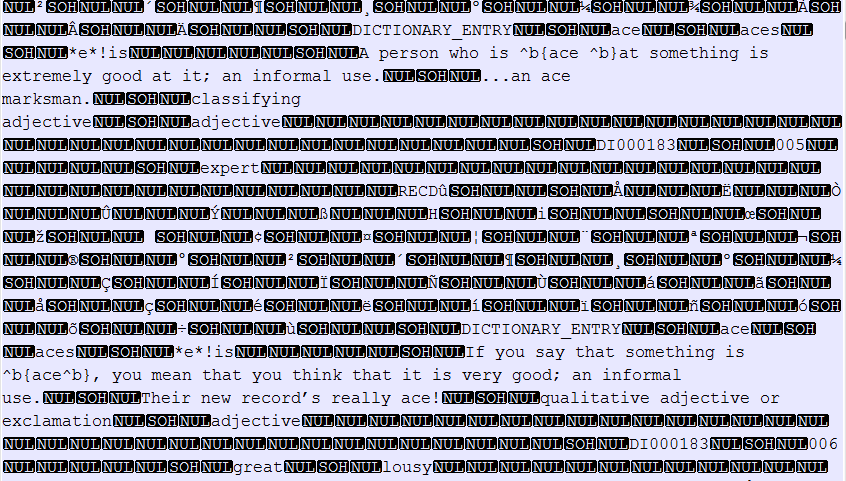
\includegraphics[width=150mm]{img/aceExample.png}
\end{center}

\noindent 

Entradas extra�das correspondientes al fragmento anterior:\\
\begin{footnotesize}
\begin{Verbatim}[samepage=true]
DICTIONARY_ENTRY
ace
aces
*e*!is    
A person who is ace at something is extremely good at it; an informal use.
...an ace marksman.
classifying adjective
adjective                                

DICTIONARY_ENTRY
ace
aces
*e*!is    
If you say that something is ace, you mean that you think that it is very good; 
an informal use.
Their new records really ace!
qualitative adjective or exclamation
adjective                                
\end{Verbatim}
\end{footnotesize}

Cada entrada arriba presentada tiene la caracter�stica de poseer una cantidad variable de campos y no es posible identificarlos exactamente. Sin embargo, contienen algunos rasgos comunes: la palabra, sus formas, la pronunciaci�n, su definici�n y uno o m�s ejemplos donde se indica como se emplea (mediante una etiqueta gramatical). 

Por ejemplo, en la primer entrada se pueden distinguir estos campos:\\

\noindent 
\begin{minipage}{\linewidth}
\begin{footnotesize}
\noindent \verb#DICTIONARY_ENTRY# \\
\verb#ace#  $\longrightarrow$ \textsl{palabra}\\
\verb#aces# $\longrightarrow$ \textsl{formas flexionadas}\\
\verb#*e*!is# $\longrightarrow$ \textsl{pronunciaci�n}\\
\verb#A person who is ace at something is extremely good at it; an informal use.# $\longrightarrow$ \textsl{definici�n}\\
\verb#...an ace marksman.# $\longrightarrow$ \textsl{ejemplo}\\
\verb#classifying adjective# $\longrightarrow$ \textsl{etiqueta espec�fica}\\
\texttt{adjective} $\longrightarrow$ \textsl{etiqueta general}\\ 
\end{footnotesize}
\end{minipage}

La siguiente tarea consisti� en procesar individualmente cada entrada identificando la palabra que se est� definiendo, las formas flexionadas de la misma y los ejemplos junto a su etiqueta gramatical asociada.

Como consecuencia se determinaron algunas caracter�sticas particulares para las entradas de Cobuild.

\begin{enumerate}
	\item Algunas entradas presentan la pronunciaci�n mientras que otras presentan detalles de la misma descriptos en lenguaje natural. Ejemplo:
	\begin{footnotesize}
	\begin{verbatim}
	DICTIONARY_ENTRY
	abstract
	abstracts, abstracting, abstracted      
	An idea, argument, or way of thinking that is abstract is based on general 
	ideas and principles rather than on particular things and events.
	The arguments of contemporary science are so abstract that they are no longer intelligible... 
	...our capacity for abstract reasoning.
	qualitative adjective
	adjective
	The word abstract is pronounced /*!abstr!akt/ when it is an adjective or a 
	noun, and /%e3bstr*!akt/ when it is a verb.  
	\end{verbatim}
	\end{footnotesize}

	\item En la mayor�a de los casos las definiciones se presentan en una sola oraci�n y en otros en m�s de una.	Ejemplo:
	\begin{footnotesize}
	\begin{verbatim}
	DICTIONARY_ENTRY
	account
	accounts, accounting, accounted
	%ek*a*!unt    
	The word account is also used in the following expressions. If you say that 
	something is the case by all accounts or from all accounts, you mean that everyone 
	you talk to about it, or everyone who writes about it, says that it is so.
	From all accounts she was a clever girl.
	phrase: used as an adjunct
	phrase                                
	\end{verbatim}
	\end{footnotesize}
\end{enumerate}

Para el caso 1, las frases explicativas sobre pronunciaci�n de las palabras fueron identificadas y descartadas, para no confundirlas con ejemplos.

Ante la imposibilidad de distinguir si una oraci�n es parte de la definici�n o un ejemplo (caso 2), se asumi� que la primera oraci�n de la entrada es la definici�n (esto es cierto en la mayor�a de los casos). 

De esta manera se evita la p�rdida de ejemplos por confundirlos con la definici�n. No obstante se introduce falsa informaci�n al identificar (en la minor�a de los casos) una oraci�n perteneciente a la definici�n como un ejemplo. Sin embargo este hecho no es tan grave: debido a las caracter�sticas de Cobuild, la palabra es generalmente definida utilizando el mismo sentido que se exhibe en el ejemplo. 

Por lo tanto se puede concluir que para la mayor�a de los casos las oraciones pertenecientes a una definici�n que se identifican como un ejemplo aportan informaci�n v�lida.
%\subsection{Nuevo Corpus generado} 
A partir del corpus parcialmente anotado obtenido en el proceso de extracci�n, se completar�n las anotaciones autom�ticamente con un etiquetador gramatical. Manteniendo las etiquetas gramaticales obtenidas a partir de la informaci�n procedente del diccionario Cobuild. Es decir, una vez finalizado el proceso de extracci�n de informaci�n desde el diccionario, se obtiene un corpus nuevo con las etiquetas gramaticales correspondientes a las palabras definiadas en el diccionario. A continuaci�n se exhibe un fragmento del mismo:\\\\

A\\
canary	NN\\
is\\
a\\
small\\
yellow\\
bird\\
which\\
sings\\
beautifully\\
.\\
People\\
sometimes\\
keep\\
canaries	NNS\\
in\\
cages\\
as\\
pets\\
.\\

Este es el resultado de extracci�n y reconocimiento de formas flexionadas correspondiente a la entrada de Cobuild: 

\begin{verbatim}
DICTIONARY_ENTRY
canary
canaries
A canary is a small yellow bird which sings beautifully. People sometimes keep
canaries in cages as pets.  
countable noun
noun                                
\end{verbatim}

Se puede apreciar que se ha reconocido \textsl{canaries} como el plural de \textsl{canary} (etiqueta NNS) y que se han reconocido y extra�do los ejemplos de estas palabras asignando las etiquetas gramaticales traducidas a partir de las etiquetas del diccionario correspondientes a \textsl{canary} (countable noun/NN) y \textsl{canaries} (noun/NNS).

Una vez realizada esta tarea, se proceder� a completar las anotaciones gramaticales para todas las palabras restantes. Este proceso se realiza anotando el corpus plano (sin las etiquetas obtenidas mediante Cobuild) con el etiquetador gramatical autom�tico TnT. Luego se une este corpus anotado totalmente con TnT con el corpus anotado parcialmente procedente de Cobuild, preservando todas las etiquetas del diccionario. El resultado que se muestra a continuaci�n es un nuevo corpus obtenido a partir de Cobuild, con las anotaciones que este provee y completado con anotaciones obtenidas mediante etiquetaci�n autom�tica utilizando TnT.\\\\

A			DT\\
canary			NN\\
is			VBZ\\
a			DT\\
small			JJ\\
yellow			JJ\\
bird			NN\\
which			WDT\\
sings			VBZ\\
beautifully		RB\\
.			.\\
People			NNS\\
sometimes		RB\\
keep			VB\\
canaries		NNS\\
in			IN\\
cages			NNS\\
as			IN\\
pets			NNS\\
.			.\\

%\subsection{Experimentaci�n} 
\subsubsection{Primer experimento} 
El primer experimento consiste en medir (generando una matriz de confusi�n) la informaci�n extra�da de COBUILD contra la misma informaci�n generada a partir de un etiquetador autom�tico (TnT). Es decir, la informaci�n extra�da de COBUILD, como se mencion� anteriormente, es la uni�n de definiciones y ejemplos, con la informaci�n gramatical correspondiente a la palabra definida.
A continuaci�n se presenta un peque�o extracto:\\
 
\begin{multicols}{2} 
\noindent A\\
cat	NN\\
is\\
a\\
small\\
furry\\
animal\\
with\\
a\\
tail\\
,\\
whiskers\\
,\\
and\\
sharp\\
claws\\
that\\
kills\\
smaller\\
animals\\
such\\
as\\
mice\\
and\\
birds\\
.\\
Cats	NNS\\
are\\
often\\
kept\\
as\\
pets\\
.\\
She\\
put\\
out\\
a\\
hand\\
and\\
stroked\\
the\\
cat	NN\\
softly\\
...\\
...\\
domestic\\
animals\\
such\\
as\\
dogs\\
and\\
cats	NNS\\
.\\
\end{multicols}
Esta es la informaci�n extra�da de COBUILD para la palabra \textsl{cat}; la uni�n de la definici�n:\\
\\
\textsl{A cat is a small furry animal with a tail, whiskers, and sharp claws that kills smaller animals such as mice and birds. Cats are often kept as pets.}\\
\\
y los ejemplos\\
\\
\textsl{She put out a hand and stroked the cat softly... }\\
\textsl{...domestic animals such as dogs and cats.}\\
\\
Se puede notar la informaci�n gramatical expresada mediante las etiquetas NN y NNS para las palabras \textsl{cat} y \textsl{cats} respectivamente.
La idea de este experimento ser� comparar estas etiquetas contra las etiquetas asignadas por el etiquetador autom�tico TnT. Entonces se tomar� este corpus plano (sin etiquetas), se lo etiquetar� utilizando TnT entrenado con el corpus de entrenamiento Wall Street Journal (de ahora en m�s WSJ) \footnote{Wall Street Journal es un corpus anotado, parte del Penn Treebank} y luego se realizar� la comparaci�n.\\
La matriz de confusi�n\footnote{Las matrices de confusi�n presentadas de aqu� en adelante contienen las primeras 10 etiquetas de mayor error} generada a partir de dicha comparaci�n es la siguiente:

\begin{center}
\begin{longtable}{| l | c | c | c | c | c | c | c | c | c | c | }
\caption{Matriz de confusi�n para etiquetas extra�das de COBUILD vs generadas por TnT}\\	
\hline
 \backslashbox{\scriptsize{COBUILD}\kern-1em}{\kern-1em \scriptsize{TnT}}  &	\textbf{NN}	&   \textbf{VB}	&   \textbf{JJ}	&   \textbf{VBN}	&   \textbf{RB}	&   \textbf{VBG}	&   \textbf{NNP}	&   \textbf{IN}	&   \textbf{VBZ}	&   \textbf{NNS}	&   \hline
\endhead
\hline
\endfoot
\endlastfoot
	\hline
\textbf{NN} & - & \textbf{556} & \textbf{1953} & 52 & 86 & 276 & - & 8 & - & -\\
\textbf{VB} & \textbf{2616} & - & \textbf{614} & - & 42 & - & 77 & 15 & - & 5\\
\textbf{JJ} & \textbf{1577} & 96 & - & \textbf{1361} & \textbf{634} & \textbf{555} & \textbf{281} & 30 & - & 16\\
\textbf{VBN} & - & - & - & - & - & - & - & - & - & -\\
\textbf{RB} & 219 & 23 & \textbf{408} & 10 & - & 9 & 34 & 249 & - & 11\\
\textbf{VBG} & - & - & - & - & - & - & - & - & - & -\\
\textbf{NNP} & - & - & - & - & - & - & - & - & - & -\\
\textbf{IN} & - & - & - & - & - & - & - & - & - & -\\
\textbf{VBZ} & - & - & - & - & - & - & - & - & - & -\\
\textbf{NNS} & 83 & 1 & 17 & - & 1 & 2 & 104 & 3 & 192 & -\\
\hline
\end{longtable}
\end{center}

\noindent Porcentaje de aciertos: 99,16\% \\
\noindent Cantidad de errores: 13082\\

Se puede apreciar un alto porcentaje de aciertos entre las etiquetas extra�das de COBUILD (99,16\%) y las etiquetas asignadas por TnT. Este porcentaje indica que la informaci�n de etiquetas extra�das de COBUILD es consistente con las producidas por TnT. La mayor�a de los errores se da en etiquetas VB, NN y JJ de COBUILD cuando son etiquetadas como NN, JJ y NN por TnT respectivamente.

\subsubsection{Segundo experimento: entrenamiento de TnT con la nueva fuente de informaci�n generada} 
El segundo experimento realizado tiene como objetivo evaluar la nueva fuente de informaci�n obtenida (NFI) como corpus de entrenamiento. Para esto se utilizar� el Wall Street Journal (WSJ), parte de Penn Tree Bank, como corpus objetivo.\\

La primer evaluaci�n de este segundo experimento consiste en entrenar el etiquetador gramatical con WSJ como corpus de entrenamiento y con WSJ + NFI. Luego se procede a etiquetar el WSJ plano (sin etiquetas gramaticales) con estos dos modelos. Por �ltimo se contruye la matriz de confusi�n:

\begin{center}
\begin{longtable}{| l | c | c | c | c | c | c | c | c | c | c | }
\caption{WSJ original contra WSJ etiquetado con TnT (entrenado con WSJ)}\\	
\hline
 \backslashbox{\scriptsize{WSJ}\kern-1em}{\kern-1em \scriptsize{TnT(WSJ)}}  &	\textbf{JJ}	&   \textbf{NN}	&   \textbf{NNP}	&   \textbf{VBN}	&   \textbf{VBD}	&   \textbf{IN}	&   \textbf{RB}	&   \textbf{RP}	&   \textbf{NNPS}	&   \textbf{VBG}	&   \hline
\endhead
\hline
\endfoot
\endlastfoot
	\hline
\textbf{JJ} & - & 909 & 717 & \textbf{932} & 51 & 71 & 569 & 23 & 1 & 229\\
\textbf{NN} & \textbf{2537} & - & \textbf{1680} & 30 & 40 & 19 & 72 & 7 & - & 622\\
\textbf{NNP} & 454 & 358 & - & 4 & 3 & 26 & 47 & 1 & \textbf{1262} & 7\\
\textbf{VBN} & \textbf{1215} & 37 & 22 & - & \textbf{1151} & - & - & - & - & -\\
\textbf{VBD} & 60 & 40 & 6 & \textbf{1522} & - & - & - & - & - & -\\
\textbf{IN} & 109 & 4 & 28 & - & - & - & \textbf{1429} & \textbf{1353} & - & 2\\
\textbf{RB} & 752 & 203 & 46 & 4 & 1 & \textbf{1500} & - & 842 & - & 1\\
\textbf{RP} & 2 & - & 1 & - & - & 371 & 144 & - & - & -\\
\textbf{NNPS} & 34 & - & 418 & - & - & - & - & - & - & -\\
\textbf{VBG} & 411 & 879 & 19 & - & - & - & - & - & - & -\\
\hline
\end{longtable}
\end{center}

\noindent Porcentaje de aciertos: 97,38\%

\begin{center}
\begin{longtable}{| l | c | c | c | c | c | c | c | c | c | c | }
\caption{WSJ original contra WSJ etiquetado con TnT (entrenado con WSJ + NFI)}\\	
\hline
 \backslashbox{\scriptsize{WSJ}\kern-1em}{\kern-1em \scriptsize{TnT(WSJ+NFI)}}  &	\textbf{JJ}	&   \textbf{NN}	&   \textbf{NNP}	&   \textbf{VBN}	&   \textbf{VBD}	&   \textbf{IN}	&   \textbf{RB}	&   \textbf{RP}	&   \textbf{NNPS}	&   \textbf{VB}	&   \hline
\endhead
\hline
\endfoot
\endlastfoot
	\hline
\textbf{JJ} & - & 895 & 1032 & 908 & 53 & 83 & 620 & 28 & 1 & 77\\
\textbf{NN} & \textbf{2776} & - & \textbf{2087} & 48 & 43 & 16 & 83 & 7 & - & 337\\
\textbf{NNP} & 361 & 256 & - & 4 & 2 & 19 & 45 & 1 & \textbf{1255} & 11\\
\textbf{VBN} & \textbf{1326} & 35 & 27 & - & \textbf{1236} & - & - & - & - & 43\\
\textbf{VBD} & 69 & 24 & 10 & \textbf{1760} & - & - & - & - & - & 42\\
\textbf{IN} & 107 & 4 & 46 & - & - & - & \textbf{1163} & \textbf{1584} & - & 3\\
\textbf{RB} & 834 & 193 & 63 & 4 & 1 & \textbf{1705} & - & \textbf{1138} & - & 50\\
\textbf{RP} & 2 & 1 & 1 & - & - & 348 & 88 & - & - & -\\
\textbf{NNPS} & 33 & - & 448 & - & - & - & - & - & - & -\\
\textbf{VB} & 89 & 408 & 34 & 48 & 42 & 13 & 11 & - & - & -\\
\hline
\end{longtable}
\end{center}

\noindent Porcentaje de aciertos: 97,12\% \\

Se puede observar que el rendimiento del etiquetador TnT entrenado con WSJ es un poco mejor (97,38\%) que el rendimiento de TnT entrenado con WSJ + NFI (97,12\%). La mayor�a de los errores para TnT entrenado con WSJ se da en etiquetas NN del gold standard cuando son etiquetadas como JJ y NNP por TnT. Para TnT entrenado con WSJ + NFI la mayor�a de los errores se da en las mismas etiquetas, pero con cantidad de errores mayor, sobre todo para NN etiquetado como JJ.\\

La segunda evaluaci�n de este experimento consiste en entrenar TnT con la mitad de WSJ y con la mitad de WSJ + NFI. Posteriormente con estos dos modelos se etiqueta la mitad restante de WSJ y se construye la matriz de confusi�n. Se realiza la misma operaci�n para cada mitad:

\begin{center}
\begin{longtable}{| l | c | c | c | c | c | c | c | c | c | c | }
\caption{Primer mitad WSJ original vs primer mitad WSJ etiquetado con TnT (entrenado con la segunda mitad de WSJ)}\\	
\hline
 \backslashbox{\scriptsize{WSJ}\kern-1em}{\kern-1em \scriptsize{TnT(2WSJ)}}  &	\textbf{JJ}	&   \textbf{NN}	&   \textbf{NNP}	&   \textbf{VBN}	&   \textbf{VBD}	&   \textbf{IN}	&   \textbf{RB}	&   \textbf{VB}	&   \textbf{VBP}	&   \textbf{RP}	&   \hline
\endhead
\hline
\endfoot
\endlastfoot
	\hline
\textbf{JJ} & - & \textbf{1042} & 547 & \textbf{810} & 54 & 20 & 312 & 61 & 6 & 6\\
\textbf{NN} & \textbf{1968} & - & \textbf{1167} & 25 & 24 & 6 & 55 & 272 & 72 & 2\\
\textbf{NNP} & 422 & 520 & - & 9 & 11 & 19 & 43 & 21 & 3 & -\\
\textbf{VBN} & 605 & 25 & 24 & - & \textbf{831} & - & - & 38 & 2 & -\\
\textbf{VBD} & 75 & 21 & 12 & \textbf{1140} & - & - & 1 & 33 & 8 & -\\
\textbf{IN} & 70 & 4 & 24 & 1 & - & - & \textbf{617} & 1 & 4 & \textbf{616}\\
\textbf{RB} & 437 & 91 & 26 & 3 & 2 & \textbf{844} & - & 19 & 3 & 316\\
\textbf{VB} & 77 & 414 & 41 & 25 & 13 & 6 & 8 & - & 343 & -\\
\textbf{VBP} & 26 & 296 & 19 & 19 & 33 & 5 & 4 & \textbf{623} & - & -\\
\textbf{RP} & - & - & 2 & - & - & 230 & 122 & - & - & -\\
\hline
\end{longtable}
\end{center}

\noindent Porcentaje de aciertos: 96,23 \%

\begin{center}
\begin{longtable}{| l | c | c | c | c | c | c | c | c | c | c | }
\caption{Primer mitad WSJ original vs primer mitad WSJ etiquetado con TnT (entrenado con segunda mitad de WSJ + NFI)}\\	
\hline
 \backslashbox{\scriptsize{WSJ}\kern-1em}{\kern-1em \scriptsize{TnT(2WSJ+NFI)}}  &	\textbf{JJ}	&   \textbf{NN}	&   \textbf{NNP}	&   \textbf{VBN}	&   \textbf{VBD}	&   \textbf{IN}	&   \textbf{RB}	&   \textbf{RP}	&   \textbf{VBG}	&   \textbf{NNPS}	&   \hline
\endhead
\hline
\endfoot
\endlastfoot
	\hline
\textbf{JJ} & - & \textbf{879} & \textbf{674} & \textbf{616} & 29 & 37 & 337 & 7 & 210 & -\\
\textbf{NN} & \textbf{1742} & - & \textbf{1293} & 29 & 27 & 6 & 65 & 2 & 560 & 1\\
\textbf{NNP} & 336 & 354 & - & 6 & 4 & 15 & 42 & - & 22 & 557\\
\textbf{VBN} & \textbf{636} & 15 & 25 & - & \textbf{716} & - & - & - & - & -\\
\textbf{VBD} & 56 & 10 & 17 & \textbf{1073} & - & - & - & - & - & -\\
\textbf{IN} & 66 & 3 & 32 & - & - & - & 506 & \textbf{750} & 2 & -\\
\textbf{RB} & 448 & 79 & 31 & 2 & 1 & \textbf{894} & - & 521 & - & -\\
\textbf{RP} & - & - & 2 & - & - & 182 & 53 & - & - & -\\
\textbf{VBG} & 309 & 467 & 23 & - & - & - & - & - & - & -\\
\textbf{NNPS} & 22 & 1 & 521 & - & - & - & - & - & - & -\\
\hline
\end{longtable}
\end{center}

\noindent Porcentaje de aciertos: 96,46\%

\begin{center}
\begin{longtable}{| l | c | c | c | c | c | c | c | c | c | c | }
\caption{Segunda mitad de WSJ original vs segunda mitad WSJ etiquetado con TnT (entrenado con la primera mitad de WSJ)}\\	
\hline
 \backslashbox{\scriptsize{WSJ}\kern-1em}{\kern-1em \scriptsize{TnT(1WSJ)}}  &	\textbf{JJ}	&   \textbf{NN}	&   \textbf{VBN}	&   \textbf{VBD}	&   \textbf{NNP}	&   \textbf{RB}	&   \textbf{IN}	&   \textbf{NNPS}	&   \textbf{RP}	&   \textbf{VB}	&   \hline
\endhead
\hline
\endfoot
\endlastfoot
	\hline
\textbf{JJ} & - & \textbf{1084} & 610 & 79 & 564 & 352 & 44 & 2 & 18 & 83\\
\textbf{NN} & \textbf{1828} & - & 36 & 30 & \textbf{1102} & 51 & 13 & - & 6 & 263\\
\textbf{VBN} & \textbf{829} & 22 & - & \textbf{874} & 30 & - & - & - & - & 34\\
\textbf{VBD} & 70 & 38 & \textbf{1107} & - & 13 & - & - & - & - & 21\\
\textbf{NNP} & 454 & 458 & 18 & 5 & - & 40 & 19 & \textbf{850} & 2 & 18\\
\textbf{RB} & 384 & 164 & 3 & - & 47 & - & \textbf{753} & - & 512 & 21\\
\textbf{IN} & 43 & 5 & - & - & 19 & \textbf{851} & - & - & \textbf{693} & 4\\
\textbf{NNPS} & 11 & - & - & - & 351 & - & - & - & - & -\\
\textbf{RP} & 2 & 1 & - & - & 1 & 85 & 227 & - & - & -\\
\textbf{VB} & 76 & 410 & 27 & 21 & 50 & 10 & 7 & - & - & -\\
\hline
\end{longtable}
\end{center}

\noindent Porcentaje de aciertos: 96,20\%

\begin{center}
\begin{longtable}{| l | c | c | c | c | c | c | c | c | c | c | }
\caption{Segunda mitad de WSJ original vs segunda mitad WSJ etiquetado con TnT (entrenado con primera mitad de WSJ)}\\	
\hline
 \backslashbox{\scriptsize{WSJ}\kern-1em}{\kern-1em \scriptsize{TnT(1WSJ+NFI)}}  &	\textbf{JJ}	&   \textbf{NN}	&   \textbf{NNP}	&   \textbf{VBN}	&   \textbf{VBD}	&   \textbf{IN}	&   \textbf{RB}	&   \textbf{RP}	&   \textbf{NNPS}	&   \textbf{VB}	&   \hline
\endhead
\hline
\endfoot
\endlastfoot
	\hline
\textbf{JJ} & - & \textbf{842} & 661 & 504 & 35 & 51 & 353 & 23 & 2 & 64\\
\textbf{NN} & \textbf{1808} & - & \textbf{1258} & 34 & 30 & 10 & 40 & 4 & - & 217\\
\textbf{NNP} & 334 & 318 & - & 14 & 8 & 11 & 27 & 1 & \textbf{783} & 18\\
\textbf{VBN} & \textbf{808} & 21 & 26 & - & \textbf{749} & - & - & - & - & 26\\
\textbf{VBD} & 46 & 16 & 13 & \textbf{1072} & - & - & - & - & - & 19\\
\textbf{IN} & 43 & 3 & 23 & - & - & - & 652 & \textbf{875} & - & 3\\
\textbf{RB} & 426 & 137 & 56 & 2 & - & \textbf{878} & - & \textbf{692} & - & 36\\
\textbf{RP} & 2 & 1 & - & - & - & 188 & 45 & - & - & -\\
\textbf{NNPS} & 15 & - & 319 & - & - & - & - & - & - & -\\
\textbf{VB} & 58 & 272 & 37 & 24 & 29 & 7 & 8 & - & - & -\\
\hline
\end{longtable}
\end{center}

\noindent Porcentaje de aciertos: 96,36\% \\

Se puede apreciar una leve mejor�a en el porcentaje de etiquetas acertadas; 96,23\% contra 96,46\% y 96,20\% contra 96,36\% para cada mitad respectivamente. Los errores m�s comunes son producidos en etiquetas NN del gold standard cuando son etiquetadas como JJ y NNP por TnT, para las dos mitades entrenadas tanto con WSJ como con WSJ + NFI. Se puede notar que el porcentaje de error al etiquetar JJ cuando era NN es menor en la evaluaci�n realizada sobre TnT entrenado con WSJ + NFI.\\

A continuaci�n se presentan las matrices de confusi�n entre la primer y segunda mitad de WSJ etiquetado con TnT entrenado con la mitad restante contra la misma mitad de WSJ etiquetado con TnT entrenado con la mitad restante + NFI.

\begin{center}
\begin{longtable}{| l | c | c | c | c | c | c | c | c | c | c | }
\caption{Primer mitad de WSJ etiquetado por TnT (entrenado con la segunda mitad WSJ) vs primer mitad WSJ etiquetado con TnT (entrenado con la segunda  mitad de WSJ + NFI)}\\	
\hline
 \backslashbox{\scriptsize{TnT(2WSJ)}\kern-1em}{\kern-1em \scriptsize{TnT(2WSJ+NFI)}}  &	\textbf{NN}	&   \textbf{JJ}	&   \textbf{VBN}	&   \textbf{VBD}	&   \textbf{NNP}	&   \textbf{VBG}	&   \textbf{VBP}	&   \textbf{VB}	&   \textbf{RP}	&   \textbf{RB}	&   \hline
\endhead
\hline
\endfoot
\endlastfoot
	\hline
\textbf{NN} & - & \textbf{567} & 32 & 19 & \textbf{458} & \textbf{334} & 108 & \textbf{319} & - & 43\\
\textbf{JJ} & \textbf{633} & - & 143 & 39 & \textbf{350} & 63 & 12 & 59 & 2 & 162\\
\textbf{VBN} & 15 & \textbf{376} & - & \textbf{443} & 7 & - & 5 & 8 & - & -\\
\textbf{VBD} & 10 & 36 & \textbf{499} & - & 13 & - & 5 & 8 & - & -\\
\textbf{NNP} & 159 & 142 & 1 & 2 & - & 6 & 3 & 18 & - & 5\\
\textbf{VBG} & 175 & 216 & - & 1 & 36 & - & - & 1 & - & 2\\
\textbf{VBP} & 94 & 2 & - & 7 & 2 & - & - & 233 & - & 3\\
\textbf{VB} & 198 & 56 & 24 & 23 & 12 & - & \textbf{326} & - & - & 1\\
\textbf{RP} & - & - & - & - & - & - & - & - & - & 6\\
\textbf{RB} & 26 & 146 & 1 & 1 & 13 & - & - & 7 & 302 & -\\
\hline
\end{longtable}
\end{center}

\noindent Porcentaje de aciertos: 98,39\% \\

\begin{center}
\begin{longtable}{| l | c | c | c | c | c | c | c | c | c | c | }
\caption{Segunda mitad WSJ etiquetado por TnT (entrenado con la primera mitad WSJ) vs segunda mitad WSJ etiquetado con TnT (entrenado con la primera mitad de WSJ + NFI)}\\	
\hline
 \backslashbox{\scriptsize{TnT(1WSJ)}\kern-1em}{\kern-1em \scriptsize{TnT(1WSJ+NFI)}}  &	\textbf{JJ}	&   \textbf{NN}	&   \textbf{VBN}	&   \textbf{VBD}	&   \textbf{NNP}	&   \textbf{RP}	&   \textbf{RB}	&   \textbf{IN}	&   \textbf{VB}	&   \textbf{VBP}	&   \hline
\endhead
\hline
\endfoot
\endlastfoot
	\hline
\textbf{JJ} & - & \textbf{510} & 195 & 43 & \textbf{319} & - & 125 & 9 & 47 & 19\\
\textbf{NN} & \textbf{729} & - & 27 & 25 & \textbf{426} & 1 & 41 & 4 & \textbf{291} & 69\\
\textbf{VBN} & \textbf{282} & 20 & - & \textbf{438} & 4 & - & 1 & - & 11 & 5\\
\textbf{VBD} & 56 & 12 & \textbf{522} & - & 3 & - & 1 & - & 8 & 3\\
\textbf{NNP} & 117 & 133 & 5 & 3 & - & - & 10 & 9 & 25 & 4\\
\textbf{RP} & - & 2 & - & - & 1 & - & 35 & 32 & - & -\\
\textbf{RB} & 160 & 35 & - & - & 35 & \textbf{353} & - & \textbf{300} & 16 & 2\\
\textbf{IN} & 2 & 2 & - & - & 14 & 159 & 73 & - & - & 1\\
\textbf{VB} & 43 & 183 & 18 & 17 & 17 & 1 & 4 & 1 & - & 275\\
\textbf{VBP} & 16 & 102 & 3 & 7 & 1 & - & 1 & 1 & 201 & -\\
\hline
\end{longtable}
\end{center}

\noindent Porcentaje de aciertos: 98,45\% \\

La tercer evaluaci�n de este experimento consiste en entrenar TnT con un cuarto de WSJ y con un cuarto de WSJ + NFI. Posteriormente con estos dos modelos se etiqueta los 3/4 restantes de WSJ y se construye la matriz de confusi�n. Se realiza la misma operaci�n para cada uno de los cuartos:

\begin{center}
\begin{longtable}{| l | c | }
\caption{Rendimiento de TnT entrenado con cuartos de WSJ con y sin NFI}\\	
\hline
 \textbf{Evaluaci�n}	&   \textbf{Porcentaje de aciertos}	&   \hline
\endhead
\hline
\endfoot
\endlastfoot
	\hline
TnT entrenado con el primer 1/4 de WSJ & 95.92\%  \\
TnT entrenado con el primer 1/4 de WSJ + NFI & 96.25\% \\
TnT entrenado con el segundo 1/4 de WSJ & 95.88\% \\
TnT entrenado con el segundo 1/4 de WSJ + NFI & 96.25\% \\
TnT entrenado con el tercer 1/4 de WSJ & 95.90\% \\
TnT entrenado con el tercer 1/4 de WSJ + NFI & 96.28\% \\
TnT entrenado con el cuarto 1/4 de WSJ & 95.89\% \\
TnT entrenado con el cuarto 1/4 de WSJ + NFI & 96.29\% \\
\hline
\end{longtable}
\end{center}

En todos los casos se puede apreciar una mejora en el acierto de etiquetas para el corpus de entrenamiento WSJ + NFI contra WSJ.\\

La cuarta evaluaci�n de este experimento consiste en entrenar TnT con un d�cimo de WSJ y con un d�cimo de WSJ + NFI. Posteriormente con estos dos modelos se etiqueta los 9/10 restantes de WSJ y se presentan los resultados:
\begin{itemize}
	\item 95.31\% de acierto de etiquetas para el etiquetado de 9/10 de WSJ con TnT entrenado con 1/10 WSJ
	\item 96.09\% de acierto de etiquetas para el etiquetado de 9/10 de WSJ con TnT entrenado con 1/10 WSJ+NFI
\end{itemize}

Se puede apreciar un aumento del porcentaje de aciertos en el corpus de entrenamiento que incorpora NFI.

\subsubsection{Tercer experimento} 
%

